% Class:
\documentclass[notitlepage]{report}

% Fonts:
\usepackage[T1]{fontenc}
\usepackage{lmodern}

% Links:
\usepackage{hyperref}

% Maths:
\usepackage{amsmath}
\usepackage{amssymb}
\usepackage{mathrsfs,amsmath}
\newcommand{\e}[1]{\times 10^{#1}}
\usepackage{siunitx}

% Algorithms:
\usepackage{algorithm}
\usepackage{algpseudocode}

% Figures:
\usepackage{graphicx}
\usepackage{caption}
\usepackage{subcaption}
\graphicspath{ {./} }
\usepackage{float}

% Footnotes:
\usepackage[symbol]{footmisc}
\renewcommand{\thefootnote}{\fnsymbol{footnote}}

% Others:
\usepackage{pdfpages}
%\usepackage[backend=bibtex]{biblatex}
\usepackage{textcomp}
\usepackage{pdflscape}
\usepackage{titling}

% Title:
\title{
	Sound-source Localisation using a Microphone-array for NUbots\\
	Interim Report
}
\author{Clayton Carlon, C3327986}
\date{\today}

% Document:
\begin{document}

%\begin{titlepage}
\maketitle
\begin{abstract}
The ability to locate a source of sound is wanted for the use on robots. A number of signal-processing techniques for an array of microphones in the literature are explored. The three kinds are time-difference of arrival (TDOA), beamforming, and multiple signal classification (MUSIC). The main considerations for the literature-review have been the robustness to noise and to reverberation, the dimensions of the array, and the embedded computation. Two examples have been evaluated in simulation, a TDOA-based and iteration-based algorithm that can estimate the full 3D position of the source, and a beamforming-based method using cross-correlation that can only find the 3D direction.
\end{abstract}
%\end{titlepage}

\tableofcontents

\chapter{Introduction}

Locating a source of sound is a long sought after ability in technology, especially in the study and development of robotics which seeks to emulate and compete with human senses. The main aspiration for this project is to develop an array of microphones along with an accompanying computation, preferably embedded, to locate a source of sound using signal-processing techniques. In the end, this system will be used on the football-playing robots in the NUbots team, the university's on-campus robotics team. Therefore, the problem for this project to solve is to develop a sound-source-localisation technique using a combination of electronics, embedded computing, and signal-processing so that the robots can locate events on the field and possibly interact with and selectively listen to humans.

\section{Background}

NUbots \footnote{https://nubook.nubots.net/} is a multidisciplinary team under the University of Newcastle's robotics research group and has competed since 2002 in RoboCup, an international competition where humanoid robots play association-football\footnote{otherwise known as football or soccer}. The team is multidisciplinary and is made up of both undergraduate and postgraduate students in computer science and engineering. At this time, the robots on the team are modified versions of the igus\textregistered\ Humanoid Open Platform; this modified platform is called the NUgus hardware platform and competes in the kid-size league.

\begin{figure}[H]
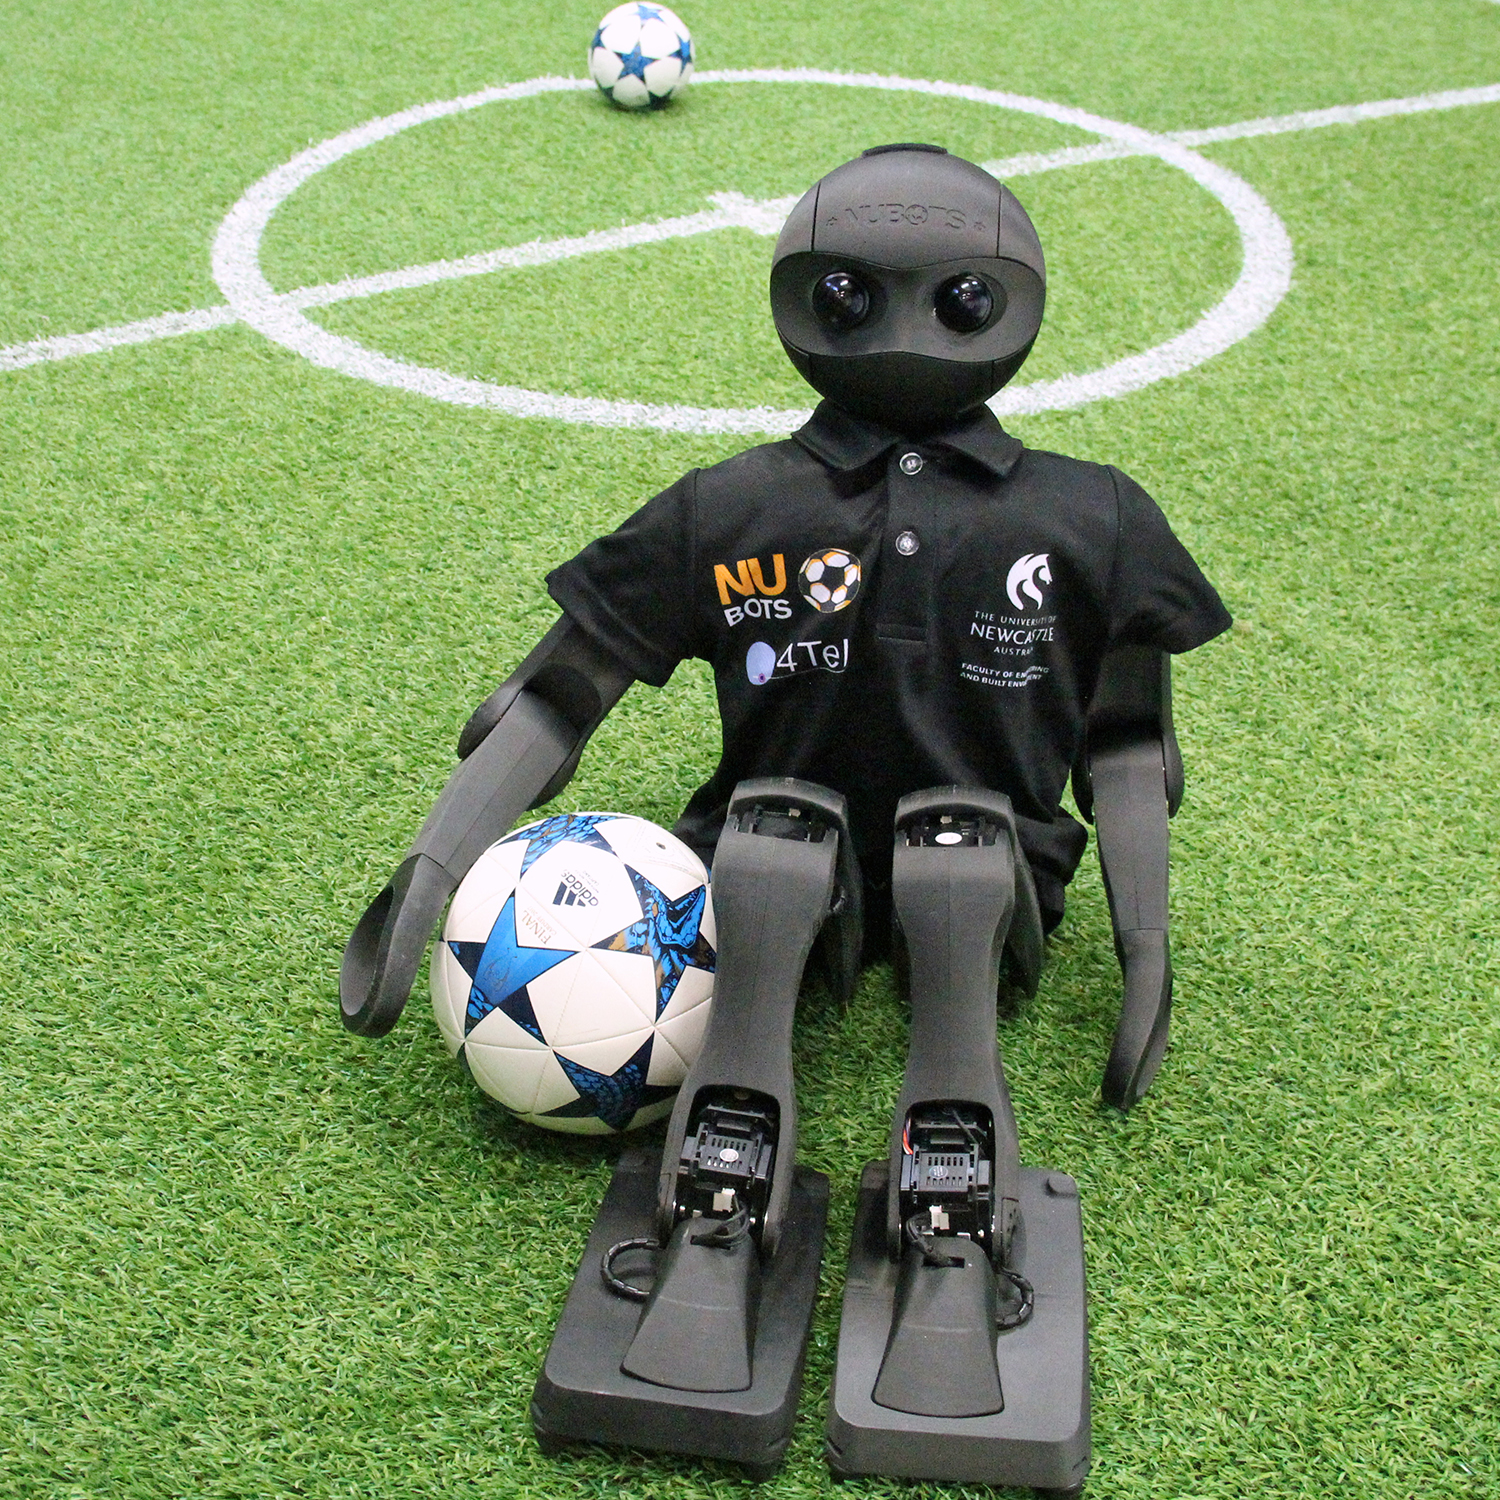
\includegraphics[width=0.75\textwidth]{./NUbot-sitting-down.jpg}
\centering
\caption{The NUgus robots are mainly used by the NUbots teams to compete in RoboCup}
\label{fig:nuguses}
\centering
\end{figure}

The remit of the team is broad and is not only competing in the RoboCup. Although it strives to win RoboCup, the team also does research more generally in areas related to robotics, such as computer-vision, robotic locomotion and control, etc. Therefore, the project does not necessarily have to be tied to the said competition. Furthermore, this project, as it evolves, does not necessarily have to be used in the application of NUbots nor robotics more generally although the original idea came from NUbots. Sound-source-localisation is a broad area of study, and the final prototype can just as easily be employed in other applications, such as a video-conference-system, drones, etc.

\section{Scope}

Ideally, the project shall yield a working prototype fitted on one of the NUgus robots. At this time, since the project is more intended as a proof-of-concept, its goals are thus somewhat open-ended. However, such basic goals are that it should at the very least:
\begin{itemize}
	\item estimate the three-dimensional direction, i.e. the azimuth and the elevation,
	\item locate a reasonably distinct sound in a moderate environment, e.g. a whistle, a lone voice, a loud thud,
	\item and handle the noise from the motors of the robot which will be nearby.
\end{itemize}
Further goals are that it can:
\begin{itemize}
	\item estimate the distance along with direction, essentially locate the source's full coordinates in three-dimensions,
	\item track the location over time using e.g. a Kalman filter,
	\item locate multiple simultaneous sources, as long as they have relatively distinct locations,
	\item spatially filter the localised sound,
	\item and work well enough in noisy and reverberant environments, e.g. in a hall full of people.
\end{itemize}

% accuracy 

Although sound-source-localisation will be helpful in a scenario of football-playing robots, the final system does not have to directly help the robot's performance in a match. The ability for a robot to interact with humans is a broad and well sought after goal. Even a basic demonstration of the robot turning its head towards a human speaker can help the team's outreach and marketing in exhibition-shows, publicity-events, etc. Not only will this help sponsors and thus funding for the team, but even the basic proof of concept also contributes further to the team's research in and remit of robotics 

\chapter{Literature-Review}

Since sound-source-localisation is a much widely researched problem, in e.g. robotics, drones, video-conferencing, the military, submarines, hearing aids, etc., the review of the literature can be quite broad. To narrow the search, and to also find examples that are most relevant to this project, especially for computation and dimensions, this review has mostly considered literature with a robotics context, rather than large-scale military outdoor application for example. Indeed, sound-source-localisation for drones shares a good deal with that for robotics, e.g. the influence of motors, but one important difference is the fact that applications for drones are mostly outdoors rather than indoors where the reverberation is an important factor.

To further help narrow the scope of the search, most methods considered are ones that use an array of at least two microphones and use some kind of classical signal-processing. Other kinds of methods exist such as binaural approaches with two microphones and head-models \cite{argentieri_survey_2015} and those that use machine-learning, such as convolutional neural networks \cite{sakavicius_multiple_2022}. It is not necessarily that these other approaches will be ignored outright but rather that the scope of the literature-review as well as the project as a whole will be kept relevant in order to ease the search and to deepen the study of a few relevant methods.

\section{Overview of Methods}

There are already a few reviews of the literature, each going through a number of existing and studied methods for sound-source-localisation. A survey \cite{argentieri_survey_2015} attempted to give a state of the art of sound-localisation in robotics. It dealt with two main areas, namely binaural approaches and array-based approaches. Since an array of microphones will be used in this project, the latter area is most relevant. All the approaches of which that the survey explored were listed as such:
\begin{itemize}
	\item MUSIC,
	\item time-difference of arrival (TDOA), and
	\item beamforming.
\end{itemize}

Another review \cite{rascon_localization_2017} also classified methodologies as:
\begin{itemize}
	\item one-dimensional single direction-of-arrival estimation,
	\item two-dimensional single direction-of-arrival estimation,
	\item multiple direction-of-arrival estimations, and
	\item distance-estimation.
\end{itemize}
Here, the review talks about correlation as a way to estimate a single direction of arrival and about beam-forming and MUSIC as a way to estimate multiple directions. It also discusses the potential use of correlation for multiple sources given that other sources are represented as secondary peaks. 

To estimate the distance, the review proposes a number of ways, some of which are:
\begin{itemize}
	\item the intersection of hyperbolic curves from multiple estimated TDOA,
	\item triangulation of multiple DOA at different positions of the robot using its mobility,
	\item triangulation of multiple DOA from different sub-arrays,
\end{itemize}

Some of the methods and approaches reviewed hereafter are only described on the surface, but some hand-picked ones are further studied in the next chapter on simulation.

\subsection{The Far Field and the Near Field}

One important distinction about the geometry is the far field and the near field. Many methods approximate their algorithm and computation by assuming that the source is in the far field where the distance between the source and the array is comparably longer than the array's width. This is such that the sound-waves may be assumed to be planar at the array and such that the direct lines between the source and each microphone may be assumed to be parallel. 

Some methods, especially those of beam-forming, can estimate distance but only in the near field where the distance between the source and the array is comparable to the array's width. However, since the microphone-arrays in robotic applications are generally small, only the far field is an acceptable assumption. This may especially be the case for NUbots where candidate space for an array on the existing NUgus is sparse, and a smaller array may have to be chosen. Thus, one must keep this distinction in geometry in mind hereafter.

\section{Time-Difference of Arrival}

A simple yet proven way to estimate the DOA of a sound-source using a microphone-array is to calculate the difference in time \cite{argentieri_survey_2015}. Commonly, the TDOA of two microphones is often found by the cross-correlation of two signals, the highest peak of which corresponds to the estimated TDOA. The cross-correlation is generally written in discrete-time as:
\begin{equation}
R_{ij}(\tau) = \sum_{n=0}^{N-1} x_i[n]x_j[n-\tau]
\end{equation}
where $x_i$ and $x_j$ are the two signals, from two microphones for example. Cross-correlation is useful in particular because it has an equivalent calculation in the frequency-domain:
\begin{equation}
R_{ij}(\tau) = \mathfrak{F}^{-1} \left( X_i[k]X_j[k]^* \right)
\end{equation}
where $X_i[k]$ and $X_j[k]$ are the Fourier transforms of $x_i$ and $x_j$ respectively. Unlike the original calculation which relies on addition and has a complexity of $O(N^2)$, this frequency-domain equivalent relies on multiplication, can be made more efficient by FFT, and has a complexity of $O\left(N\ln(N)\right)$ \cite{valin_robust_2003}.

An advanced form of this TDOA estimation is the generalised cross-correlation (GCC):
\begin{equation}
R^{(w)}_{ij}(\tau) = \mathfrak{F}^{-1} \left( \psi[k]X_i[k]X_j[k]^* \right)
\end{equation}
where $\psi[k]$ is the spectral weighting \cite{argentieri_survey_2015}, \cite{rascon_localization_2017}. A common weighting is the phase-transform (GCC-PHAT):
\begin{equation}
\psi[k] = \frac{1}{\lvert X_i[k] \rvert \lvert X_j[k] \rvert}
\end{equation}
which whitens the signals and emphasises only information on the phases rather than the magnitudes.

The TDOA can therefore be estimated as the point in time where the GCC-PHAT is highest:
\begin{equation}
\Delta t_{ij} = \text{argmax}_\tau \left( R^{(w)}_{ij} (\tau) \right)
\end{equation}

Given the TDOA $\Delta t_{ij}$, and assuming that the source is far enough, the two-dimensional angle of arrival at a pair of microphones can be estimated from simple trigonometry of parallel lines:
\begin{equation}
\theta = \sin\left( \frac{c\Delta t_{ij}}{d_{ij}} \right)
\end{equation}
where $c$ is the speed of sound, and $d_{ij}$ is the displacement between the microphones, and assuming that the source is in the far field.

The former expression is the most basic approach for a simple two-dimensional estimation of a single angle, often the azimuth. There are of course more sophisticated examples of finding the source three-dimensionally, even with distance. In fact, more generally, the given TDOA draws a hyperbola as the locus of possible positions on the two-dimensional plane (a hyperboloid in the three-dimensional case) where the two microphones are the foci of such a hyperbola. This hyperbola can be seen as a straight line in the far field.
% figure for the hyperbola?

Another important consideration is the resolution. Since the cross-correlation is a time-domain signal whose resolution is the sample-period of the two input signals, then the estimated TDOA is a multiple of the sample-period \cite{argentieri_survey_2015}. This thus yields a resolution on the estimated angle which is worst when the source is in line with the microphones. One way to improve the resolution is to interpolate the signal, i.e. growing the number of samples of the signal. Another way is to simply sample faster, but this may make the computation more burdensome.

\subsection{Distance}

The estimation of distance is not very common in TDOA-based methods. Most examples only localise the direction, whether it is two-dimensional or three-dimensional. As said before, the TDOA yields a hyperbola or hyperboloid as the locus of the source. Therefore, a naive method would be to find the intersection given at least two pairs of microphones. However, error and noise of course make this hard as well as the computation in a robotics context \cite{rascon_localization_2017}.

Another way is to use two or more sub-arrays that yield single DOAs and are used to triangulate on a position \cite{rascon_localization_2017}. However, such a method would need sub-arrays that are far apart enough which is hard for a small robot where space is a luxury.

% The review has a few examples?

\subsection{Reverberation}

Reverberation is a big influence on the estimation of TDOA, especially in a room, since it leads to delayed reflections of the signal which show up in the GCC-PHAT. A statistical analysis \cite{gustafsson_source_2003} showed that the PHAT is the best estimator for the TDOA. The numerical examples in the paper showed good results as long as the reverberation-time was more than 0.07 \si{s}, the displacement between the microphones is longer than 0.2 \si{m}, and the distance between the source and the microphones is longer than 1.5 to 2 \si{m}. The same examples also showed that the probability of outliers was "tolerable" for a SRR more than 0 \si{dB}.

Another analysis \cite{brandstein_robust_1997} simulated three methods of estimating the TDOA, namely GCC-PHAT, GCC-ML, and Biweight. For all three, both the percentage of anomalies and the RMS error worsened for a reverberation-time longer than 0.1 \si{s}.

However, although GCC-PHAT generally handles reverberation well, it does not handle noise well across the spectrum since the algorithm gives all frequencies equal weight \cite{valin_robust_2003}. It especially does not do well with narrowband signals such as tones or voice which take up a small section of the spectrum.

% noise as a separate section

\subsection{Multiple Sources}

Although the localisation of multiple sources has been explored for other methods such as beam-forming, it has not been explored much in TDOA-based methods. This is since most examples in the literature have been built on top of the basic idea of a single peak in the GCC-PHAT. However, the relationship between secondary peaks in the cross-correlation and other sources has been discussed.

Only a few basic studies in the fundamental relationship were done. A convention paper \cite{clifford_calculating_2010} proposed a method in the context of audio-engineering where multiple sources manifested themselves as distinct peaks in the GCC-PHAT. The results showed an accuracy of at least 85 \% where the SNR is at least 46.5 \si{dB}. However, the paper only considered the estimation of the TDOA in the context of musical instruments, not localisation, and the experiment was performed with little reverberation in mind. Another analysis \cite{kwon_analysis_2010} derived the mathematical cross-correlation function based on GCC-PHAT for multiple sources but did not seem to give much experimental data. 

Even so, no literature examples were found that exploited this relationship of secondary peaks for localisation in robotics \cite{rascon_localization_2017}. However, some studies have lately developed algorithms albeit not in a robotics context. A paper \cite{brutti_multiple_2010} proposed a method where an acoustic map, such as GCF or SRP-PHAT, is used to find the most dominant source which is then de-emphasised by lessening the GCC-PHAT at the time-delay corresponding to that source; this is repeated for the next most dominant source until all others are located. However, the paper only tested this method for the near field.

Another paper \cite{boora_tdoa-based_2020} proposed a method of a delay density map made up of cubic subvolumes each of which weighted by a likelihood that a source is in it. The tested system had a resolution of 0.2 \si{m} and an RMS error at worst of about 0.6 \si{m} at an SNR of 5 \si{dB}. The experiments were tested for both the near field and the far field as well as for different arrays. The reverberation-times at 60 \si{dB} in such experiments were tested from 0.11 to 0.55 \si{s}. It also compared its own method with that of GCF-D (GCF De-emphasised) where theirs performed better.

Even given a method that only locates a single source at a time, one other way to find multiple sources is to cluster multiple estimated DOAs over many time-windows or frames. One paper \cite{rascon_lightweight_2015} does such by tracking sources with a threshold on angle and smoothing such tracking with a Kalman filter. An adaptive variation of the K-mean++ algorithm has also been used to cluster multiple sources in an aforesaid paper \cite{hu_estimation_2009}.

\subsection{Literature Examples}

\subsubsection{Valin et al., 2003, Robust Sound Source Localization Using a Microphone Array on a Mobile Robot}

The usage of TDOA in sound-source-localisation in robotics is a widely researched area. Despite the simplicity of estimating the azimuth, there are many more sophisticated methods of estimating the direction or even the position. For example, one method \cite{valin_robust_2003} solves a set of simultaneous equations from at least five microphones using the pseudo-inverse of a matrix; this yields a vector giving the three-dimensional direction. It also uses a different weighting than GCC-PHAT which gives more weight to areas of the spectrum where the SNR is higher. 

The experiment was performed with eight microphones in an open rectangular prism ($0.5\times 0.4\times 0.36$ \si{m}) on top of a mobile robot as seen in Figure-\ref{fig:valin_2003_robot} "in a room with a relatively high noise level mostly due to several fans in proximity" with "moderate" reverberation. The computation was done on a desktop PC and used about 15\% of the CPU. Three sounds were tested, speech, snap of fingers, and tap of boot. The results showed an estimated direction that degraded as the source got nearer to the array as seen in Figure-\ref{fig:valin_2003_plot}; the mean-square-error was at best 0.6 and at worst 4.9 degrees with the distance being from 0.3 to 5 \si{m}. This degradation was most likely because of the far-field assumption. The system works "properly" between 3 and 5 \si{m} although the authors claimed this as a result of "the noise and reverberation conditions". They also said that broadband signals were detected better than narrowband ones like tones.

\begin{figure}[H]
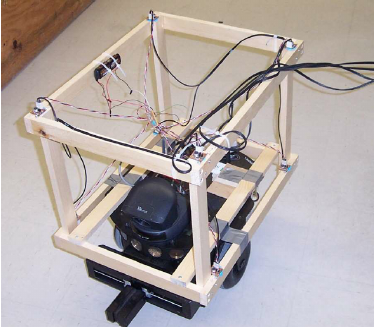
\includegraphics[width=0.75\textwidth]{./valin_2003/robot.png}
\centering
\caption{The microphone array on top of the mobile robot in \cite{valin_robust_2003}}
\label{fig:valin_2003_robot}
\centering
\end{figure}

\begin{figure}[H]
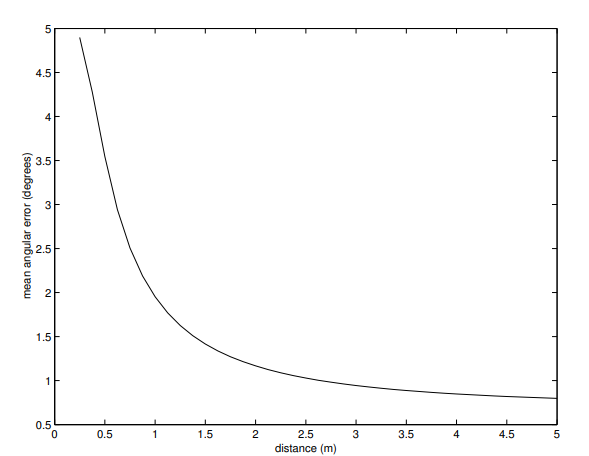
\includegraphics[width=0.75\textwidth]{./valin_2003/plot.png}
\centering
\caption{The mean angular error as a function of the distance between the source and the array in \cite{valin_robust_2003}}
\label{fig:valin_2003_plot}
\centering
\end{figure}

\subsubsection{Hu et al., 2009, Estimation of Sound Source Number and Directions Under a Multi-Source Environment}

A similar approach \cite{hu_estimation_2009} proposed a novel estimation of the TDOA, namely eigenstructure-based GCC (ES-GCC) which can handle an unknown number of multiple sources. This paper could compute as before the three-dimensional bearing but also the distance for the near-field case, i.e. when the source is near enough to the array. The K-means++ algorithm was used to cluster accumulated results. 

This approach was tested on an array of eight microphones forming a rhomboidal prism seen in Figure-\ref{fig:hu_2009_plot}; the diagonal distances from the centre were 0.22 and 0.14 \si{m}. This was done in a real room for both a single source and multiple ones that were all 2.4 \si{m} away from the array. The worst SNR was 14.58 \si{dB}. The mean error for all experiments was less than 3 \si{\deg}. The estimation of distance was not evaluated, only the azimuth and elevation. The computation was not discussed nor was reverberation.
% multiple sources?

\begin{figure}[H]
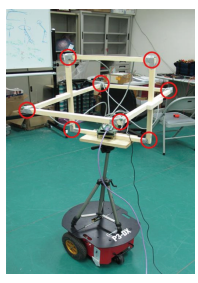
\includegraphics[width=0.75\textwidth]{./hu_2009/array.png}
\centering
\caption{The microphone array in \cite{hu_estimation_2009}}
\label{fig:hu_2009_plot}
\centering
\end{figure}

\subsubsection{Chen \& Xu, 2019, A Sound Source Localization Device Based on Rectangular Pyramid Structure for Mobile Robot}

However, the former methods only compute the bearing, at least for the far field which is more relevant for the case with a smaller array. Another example \cite{chen_sound_2019} estimates the full three-dimensional coordinates of the source by an iterative algorithm based on Newton's method to solve a set of spatial coordinate-relations. This example also had a few improvements such as a partitioning process, a fast search-strategy of the GCC peak, a screening strategy, and a new weighting function in the GCC that dealt with reverberation. However, this proposed weighting function needed beforehand the parameters of the environment and the rough displacement of the source; the authors have admitted that this limits the universality. In simulations, the improved weighting function gave a better distinct peak in the GCC for a reverberation-time of 300 \si{ms}. 

This method was tried on an array of five microphones forming a rectangular pyramid 0.25 \si{m} wide and 0.125 \si{m} tall as seen in Figure-\ref{fig:chen_2019_array}. The performance was tested at different points around the array from 1 to 6 \si{m} and with a SNR of 45 \si{dB}. The error in distance increased as the source was further away; this was observed at best as 0.05 \si{m} and at worst as 0.25 \si{m}. The error in azimuth varied little in both distance and bearing and was observed as being within 1.5 \si{\deg}. The performance was also tested at different levels of SNR, from 40 to 10 \si{dB}. In the worst case of 10 \si{dB}, the error in distance was observed at worst as 0.4 \si{m} seen in Figure-\ref{fig:chen_2019_distance_SNR}. The paper neglected any evaluation of the estimated elevation, considering that the geometry of the array is not symmetrical. Furthermore, the computational needs were not discussed in depth.

\begin{figure}[H]
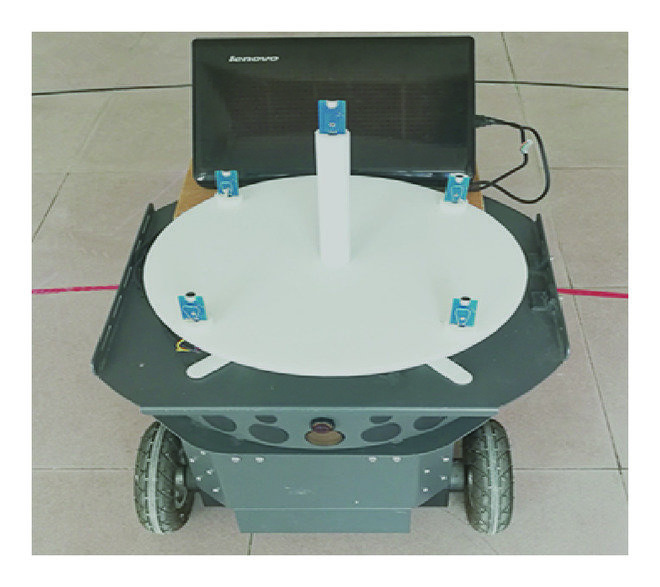
\includegraphics[width=0.75\textwidth]{./chen_2019/array.jpg}
\centering
\caption{The microphone array in \cite{chen_sound_2019}}
\label{fig:chen_2019_array}
\centering
\end{figure}

\begin{figure}[H]
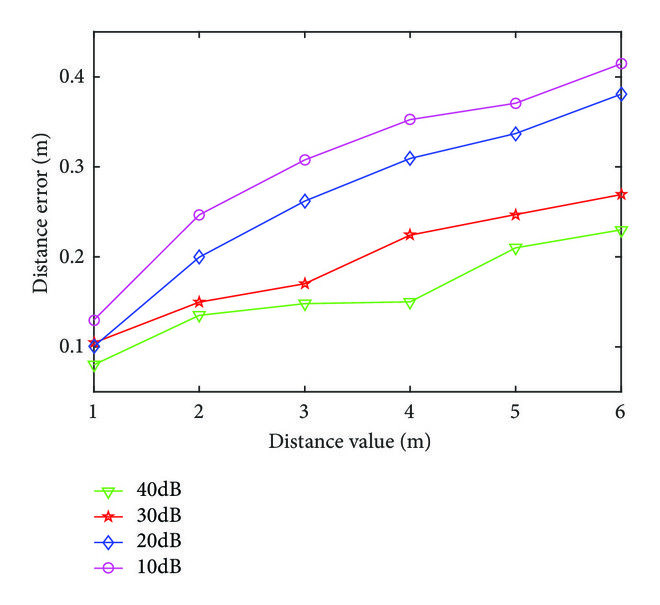
\includegraphics[width=0.75\textwidth]{./chen_2019/distance_SNR.jpg}
\centering
\caption{The error in distance as a function of distance for different SNRs in \cite{chen_sound_2019}}
\label{fig:chen_2019_distance_SNR}
\centering
\end{figure}

\subsubsection{Bechler et al., 2004, System for Robust 3D Speaker Tracking Using Microphone Array Measurements}

A similar paper \cite{bechler_system_2004} solved a similar set of equations but using Lagrange multipliers instead. It also applied tracking filtering such as an EKF. This approach was tested on an array of five microphones forming a double equilateral tetrahedron with sides 28 \si{cm} long. The SNR of the room was 15 \si{db}, and the room's reverberation-time at 60 \si{dB} was measured as 0.36 \si{s}. A number of sessions were tried where a speaking person moved along a different path. The mean squared error of the raw estimated position before filtering was observed to be at best 4.957 \si{\e{-3}}{$m^2$} and at worst 27.21 \si{\e{-3}}{$m^2$}. However, all the sessions had the speaker within 1 \si{m} of the array; so, they may be thought of as in the near field. Also, the paper makes no evaluation of the computation.

\subsubsection{Kim et al., 2008, Robust Estimation of Sound Direction for Robot Interface}

Likewise, another paper \cite{kim_robust_2008} employed robust spatial filtering, namely a Kalman filter, but only to estimate the azimuth. It used GCC-PHAT to estimate the TDOA but also used a trained feed-forward network of a single hidden layer to quantify the reliability of the estimated TDOA.

\subsubsection{Manamperi et al., 2022, Drone Audition: Sound Source Localization Using On-Board Microphones}

Potential unwanted noise from servo-motors, etc., may affect and disrupt how well the system localises wanted sources. A very recent study \cite{manamperi_drone_2022} set out an approach that estimated the azimuth and elevation and mitigated the noise from a drone's motors. Here, the authors computed the GCC-PHAT as an angular spectrum for many pairs of microphones and summed each pair's angular spectra; this method is similar to SRP-PHAT in that the azimuth and the elevation corresponding to the largest sum belong to the estimated direction. In order to mitigate the motors' noise, the authors subtracted the known angular spectrum of the drone's motors from the mixed angular spectrum before summing. This known angular spectrum was computed from noise-only recordings with specific parameters of motor's current and speed. 

The tested drone had fifteen pairs of microphones seen in \ref{fig:manamperi_2022_array} and was tested in a semi-anechoic chamber with a reverberation-time of 20 \si{ms} at 20 \si{dB}. The drone was held resting at a height of 1 \si{m} above a circle of twelve sound-sources with a radius of 0.6 \si{m}. As seen in Figure-\ref{fig:manamperi_2022_map_n30}, the results showed acceptable accuracy of the proposed method compared to that of GCC-PHAT and of MUSIC for a SNR of at least -30 \si{dB}. The experiments were performed for multiple scenarios such as for a single source and for multiple.
% May be better in beamforming?

\begin{figure}[H]
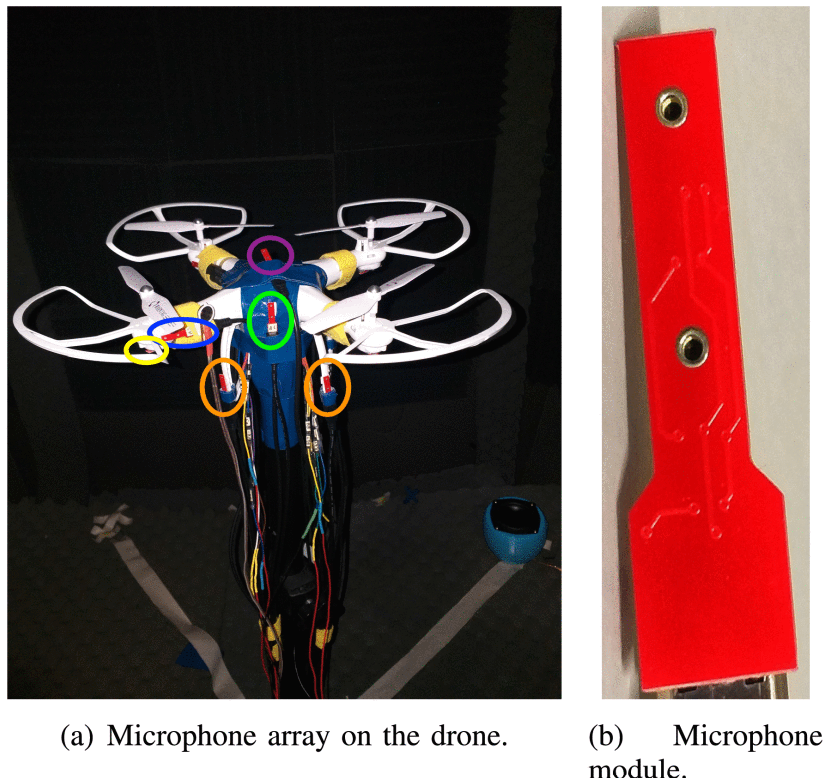
\includegraphics[width=0.75\textwidth]{./manamperi_2022/array.png}
\centering
\caption{The microphone array on the drone (a) and each pair (b) in \cite{manamperi_drone_2022}}
\label{fig:manamperi_2022_array}
\centering
\end{figure}

\begin{figure}[H]
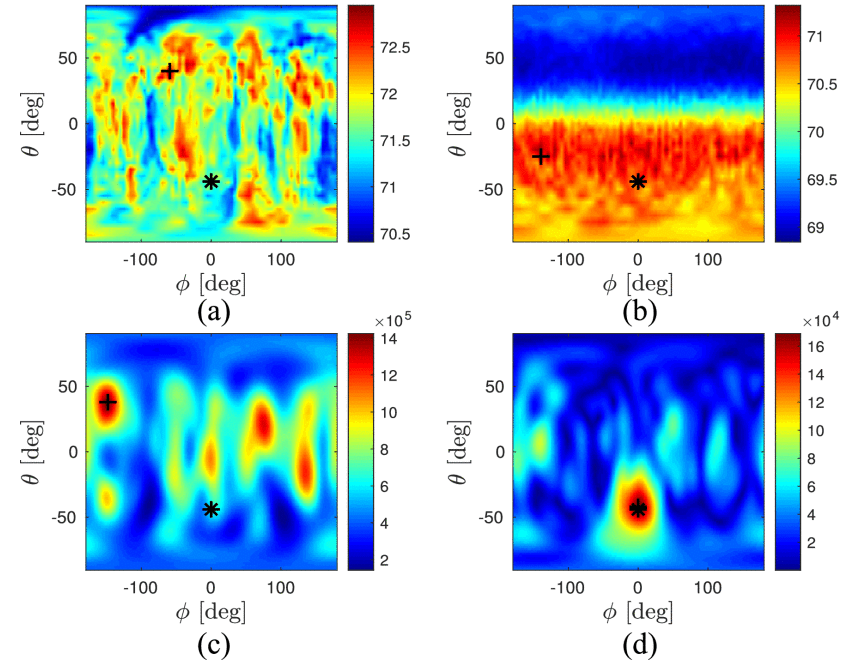
\includegraphics[width=0.75\textwidth]{./manamperi_2022/map_n30.png}
\centering
\caption{The energy maps for MUSIC (a), GEVD-MUSIC (b), GCC-PHAT (c), and the proposed method (d) at an SNR of -30 \si{dB} in \cite{manamperi_drone_2022}}
\label{fig:manamperi_2022_map_n30}
\centering
\end{figure}

\subsubsection{Mahajan \& Walworth, 2001, 3D Position Sensing Using the Differences in the Time-of-Flights from a Wave Source to Various Receivers}

Both two-dimensional and three-dimensional localisation was proposed in a paper \cite{mahajan_3d_2001} where a similar set of equations was solved, and the speed of sound could be estimated as a variable with at least six microphones. Where it was assumed to be constant, at least five microphones were needed instead. Only the two-dimensional case was evaluated in the preliminary testing. In which, the relative error in distance stayed below 1\%, and the worst error was 7.6 \si{mm} at 1 \si{m}, but this experiment was only done in a workspace $1000\times 1000$ \si{mm} and was done with ultrasonic pulses of 75 \si{kHz}. The authors did not reveal the geometry of the array and given how short the tested distances were, it may be assumed that the experiment was in the near field.

\section{Beam-forming}

Beam-forming is a common technique in signal-processing and in many applications for both sound and radio. It is a method of setting many sensors or transmitters in such an array that waves at particular angles and areas constructively interfere to form a beam focused either on a chosen spot or in a chosen direction. Traditionally, it has been used in telecommunications so that multiple radio antennae form a beam that selectively transmits only in one direction. Here, for sound-source-localisation, it is used to steer a beam or a focus in a chosen direction or on a chosen spot so that the energy only from that location is measured. If the beam is steered in enough directions, then an energy map as a function of direction, e.g. azimuth, is made. Another use that may be on interest in this project is that it can be used to spatially filter in a given direction.

One advantage of beamforming over basic localisation through TDOA is that multiple sources can be easily located since the method spatially filters, i.e. it only receives signals from a particular direction or space \cite{rascon_localization_2017}. However, if two sources are near enough to each other, then the resolution of the energy-map may not distinguish the two.

However, there are few considerations \cite{argentieri_survey_2015}:
\begin{itemize}
	\item The more microphones there are, the fewer side lobes or beams there are which show up beside the main lobe or beam.
	\item The further apart the microphones are, the narrower the beam is; this is particularly a problem for robotics where the room on a robot for an array is small.
	\item The beam from the delay-and-sum beamformer is wider at lower frequencies; this affects the resolution and precision for locating sources of lower frequencies.
	\item Copies of the main lobe appear for high frequencies; this is a form of spatial aliasing. A Shannon spatial sampling theorem is given as $d<c/(2f_{\text{max}})$ \cite{argentieri_survey_2015}.
\end{itemize}

\subsection{Delay-and-Sum}

The simplest kind of beamforming is delay-and-sum beamforming where the signal from each microphone is delayed such that the overall sum of all the delayed signals corresponds to a steered direction \cite{rascon_localization_2017}. This sum is maximum when it is steered towards the source. The delay-and-sum beamformer's output steered at the position $\vec{r}_0$ for $M$ microphones is given as the average power:
\begin{equation}
y_{\vec{r}_0}[t] = \sum_{m=1}^M x_m[t-\tau_m(\vec{r}_0)] 
\end{equation}
where $x_n$ is the signal from the $m$-th microphone, and $\tau(\vec{r}_0)$ is the time-delay at the $m$-th microphone corresponding at the position $\vec{r}_0$ \cite{argentieri_survey_2015}. In the far field, this output can be simplified to a direction, e.g. $\theta_0$ or $\vec{u}$, instead of a position:
\begin{equation}
y_{\theta_0}[t] = \sum_{m=1}^M x_m[t-\tau_m(\theta_0)] 
\end{equation}
This output can yield an energy-map as:
\begin{equation}
E_{\vec{r}_0} = \sum_{t=1}^T y_{\vec{r}_0}[t]^2
\end{equation}
or
\begin{equation}
E_{\theta_0} = \sum_{t=1}^T y_{\theta_0}[t]^2
\end{equation}

Given a direction $\vec{u}_0$, the expected TDOA can be computed as:
\begin{equation}
\Delta t_{ij} = \tau_{i}(\vec{u}_0) - \tau_{j}(\vec{u}_0) = \frac{f_s}{c} \left( \vec{r}_i - \vec{r}_j \right) \cdot \vec{u}_0
\end{equation}
where $f_s$ is the sampling frequency, $c$ is the speed of sound, $\vec{r}_m$ is the position of the $m$-th microphone. \footnote{One must keep in mind that this is not same as the TDOA estimated from the GCC-PHAT in TDOA-based methods. In fact, this particular method of beamforming highlights the subtle relationship between the two methods, namely TDOA-based and beamforming.}

A more general kind of beamforming is filter-and-sum beamforming where the signal from each microphone is filtered by its own linear filter rather than delayed \cite{argentieri_survey_2015}. The beamformer's output is given as:
\begin{equation}
y_{\vec{r}_0}[t] = \sum_{m=1}^M w_m(\vec{r}_0)[t]x_m[t]
\end{equation} 
where $w_m(\vec{r}_0)[t]$ is the impulse-response of the $m$-th linear filter.

\subsection{Steered Response Power}

Indeed, the beamformer energy can be computed in a different way using the cross-correlations of many microphones \cite{valin_localization_2004} \cite{valin_robust_2007} \cite{argentieri_survey_2015} \cite{rascon_localization_2017}. This has often been called the steered response power (SRP) and allows faster computation and spectral weighting \cite{badali_evaluating_2009}. 

As said before, the delay-and-sum beamformer is written as:
\begin{equation}
y_{\vec{u}_0}[t] = \sum_{m=1}^M x_m[t-\tau_m(\vec{u}_0)] 
\end{equation}
where $x_m$ is the signal from the $m$-th microphone, and $\tau_m(\theta)$ is the time-delay at the $m$-the microphone from the source given a direction $\vec{u}$ in the far field. This output can yield an energy-map as:
\begin{equation}
E_{\vec{u}} = \sum_{t=1}^T y_{\vec{u}_0}[t]^2
\end{equation}
given a frame $T$ samples long. This can be rewritten in terms of cross-correlations:
\begin{equation}
\begin{split}
E_{\vec{u}} &= \sum_{t=1}^T \left( \sum_{m=1}^M x_m[t-\tau_m(\vec{u}_0)] \right)^2 \\
&= \sum_{m=1}^{M} \sum_{t=1}^T x_m[t - \tau_m(\vec{u}_0)]^2 \\
&+ 2 \sum_{m_1=1}^M \sum_{m_2=1}^{m_1-1} 
\sum_{t=1}^T x_{m_1}\left(t - \tau_{m_1}(\vec{u}_0)\right) x_{m_2}\left(t - \tau_{m_2}(\vec{u}_0)\right) \\
E_{\vec{u}} &= K 
+ 2 \sum_{m_1=1}^M \sum_{m_2=1}^{m_1-1} R_{m_1,m_2} (\tau_{m_1}(\vec{u}_0) - \tau_{m_2}(\vec{u}_0))
\end{split}
\end{equation}
where $R_{ij}$ is the cross-correlation between the $i$-th and the $j$-th microphone, and $K = \sum_{m=1}^{M} \sum_{t=1}^T x_m[t - \tau_m(\vec{u}_0)]^2$ is nearly constant \cite{valin_localization_2004} \cite{valin_robust_2007}. 

Therefore, the beamformer's energy can be simply computed as the sum of cross-correlations for all pairs of microphones. Since the cross-correlation can be computed in the frequency-domain as talked about before, then a spectral weighting can be used, and other techniques used in estimating the TDOA such as GCC-PHAT can also be used. In fact, SRP with PHAT is known as SRP-PHAT.

\subsection{Frequency and Width}

As said before, the beam's shape is affected by the frequency of the received sound. Especially, the lower the frequency is the wider the beam is. This is a problem undergone in \cite{tamai_three_2005} where the band of observed frequencies has to be narrow, between 1 and 3 \si{kHz}. A frequency-invariant broadband beamformer using convex optimisation is proposed by a group for the far field \cite{argentieri_experimental_2005}, \cite{argentieri_prototyping_2005} and for the near field \cite{argentieri_modal_2006}.

% peak is affected by SIR.

% high computation

\subsection{Literature Examples}

\subsubsection{Valin et al., 2004, Localization of Simultaneous Moving Sound Sources for Mobile Robot Using a Frequency- Domain Steered Beamformer Approach}

A robotic implementation \cite{valin_localization_2004} was done where the beamformer's energy was calculated as the SRP in the frequency-domain using the cross-correlation weighted similarly to the authors' work with estimating the TDOA \cite{valin_robust_2003}. The authors claim that the spectral whitening before computing the beamformer's energy helps narrow the peaks. Here, the authors also proposed a spherical search-grid of 2562 points seen in Figure-\ref{fig:valin_2007_grid} where the beamformer's energy of each is computed. This grid yields a resolution of about 2.5 \si{\deg}. The direction, i.e. both the azimuth and the elevation, of the loudest source is found when the beamformer's energy is maximum. Thereafter, the cross-correlation is zeroed for that loudest source, and the search is repeated for the next loudest source. This is done for a predicted number of sources. If there are fewer sources than the set number, then a source is falsely detected. To handle this, the authors employed probabilistic post-processing to temporally smooth the estimations. Furthermore, in their experiments, they applied two estimators working together, namely a short-term estimator for two sources and a medium-term one for four. 

The experiments were performed with with eight microphones in an open rectangular prism ($0.5\times 0.4\times 0.36$ \si{m}) on top of a mobile robot in "a noisy environment with moderate reverberation"; in fact, this is the same array and robot in the authors' former work \cite{valin_robust_2003} as seen before in Figure-\ref{fig:valin_2003_robot}. The computation was done on a desktop PC and used about 30\% of the CPU. Firstly, the detection-rate was tested against distance for three kinds of sounds, namely hands clapping, speech, and a burst of white noise 250 \si{ms} long. The system was able to detect these sounds reliably up to 5 \si{m}, but drops around 7 \si{m}. The authors claimed that narrowband signals such as tones and speech were detected worse, whilst those with a broader band, such as noise, could be detected much better at longer distances. Furthermore, the estimated azimuth was accurate for four moving speakers although struggled to detect seven. Similar accuracies for both the azimuth and the elevation were given when the robot was moving instead; the authors claim that this demonstrates the robustness against the noise of the motors. Lastly, the array was shown to still be able work when it was not completely open.

\begin{figure}[H]
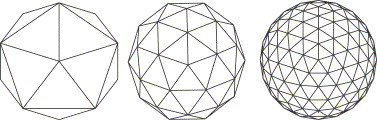
\includegraphics[width=0.75\textwidth]{./valin_2007/grid.jpg}
\centering
\caption{The evolution of the search-grid of 2562 points used in \cite{valin_robust_2003} and in \cite{valin_robust_2007}}
\label{fig:valin_2007_grid}
\centering
\end{figure}

\subsubsection{Valin et al., 2007, Robust Localization and Tracking of Simultaneous Moving Sound Sources Using Beamforming and Particle Filtering}

The same authors later used the same beamforming method but with a particle filter instead \cite{valin_robust_2007}. It also involved a refined search after detecting a source that also estimated distance, but this estimated range was found to be too unreliable. It did however improve the accuracy of the direction in the near field. This new approach was tested on two different arrays on a different mobile robot seen in Figure-\ref{fig:valin_2007_array}. The first array, C1, was an open cube of eight microphones 15.5 \si{cm} wide, whilst the second, C2, was a closed square of four about 40 \si{cm} wide on the robot's chest. 

The experiments were tested in two different environments; the first environment, E1, was a medium-sized room with a reverberation time of 350 \si{ms} at - 60 \si{dB}, whilst the second, E2, was a hall with a reverberation-time of 1.0 \si{s}. In the first environment E1, the open array C1 detected sources more reliably than the closed array C2 within seven metres; C2 struggled to detect hand-claps specifically. Again, in E1, the RMS error for both the azimuth and the elevation was at worst 1.10 \si{\deg} for C1 and at worst 1.44 \si{\deg}. As before, experiments where either multiple sources were moving or the robot was moving were tested in both E1 and E2 as well as where the trajectories of two sources intersect. In such results, the system was deemed to track successfully as seen in Figure-\ref{fig:valin_2007_track}. 

Unlike the one before, this paper also discusses the computation needed, namely for the cross-correlation. For 1024 samples at 48 \si{kHz}, eight microphones, and 2562 searched directions, the complexity is claimed to be only 48.4 \si{Mflops} after counting all time-frequency transformations.

\begin{figure}[H]
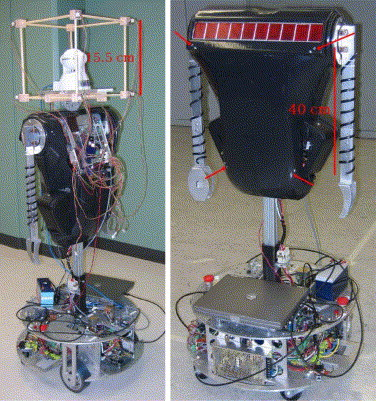
\includegraphics[width=0.75\textwidth]{./valin_2007/array.jpg}
\centering
\caption{The two different microphone arrays on the mobile robot, namely C1 on the left and C2 on the right, tested in \cite{valin_robust_2007}}
\label{fig:valin_2007_array}
\centering
\end{figure}

\begin{figure}[H]
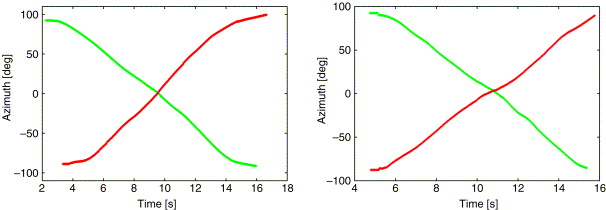
\includegraphics[width=0.75\textwidth]{./valin_2007/track.jpg}
\centering
\caption{The estimated azimuth of two tracked sources crossing paths tested in E1 on the left and in E2 on the right in \cite{valin_robust_2007}}
\label{fig:valin_2007_track}
\centering
\end{figure}

\subsubsection{Badali et al., 2009, Evaluating Real-Time Audio Localization Algorithms for Artificial Audition in Robotics}

A further study \cite{badali_evaluating_2009} compared different variations and strategies of this kind of beamforming as well as the classic estimation of TDOA through GCC-PHAT. Here, TDOA-estimation from the peak of the GCC-PHAT (PEAK) was compared against a classic beamformer, called the steered-response-power (SRP) by the authors. Two variations were also considered, namely spectral weighting (SW) against SNR as proposed in \cite{valin_robust_2003}, \cite{valin_localization_2004}, \cite{valin_robust_2007} and direction-refinement (DR) as also studied in \cite{valin_robust_2007}. The latter is where a local search with a finer resolution is done after the initial search. Furthermore, two search grids are compared, namely a spherical rectangular grid (R) tessellated at 3600 points and a triangular element grid (T) of 2562 points. A cubical array of eight microphones with dimensions of 32 by 32 by 36 \si{cm} seen in Figure-\ref{fig:badali_2009_array} was tested. 

The experiments were done in a room with a reverberation-time of 0.1 \si{s}. The source playing pre-recorded sequences of speech was set at five points of different angle and distance as well as at two heights, one level with the robot and the other at the height of a human. The SNR received was varied by lowering the volume of the source. Two distinct experiments were done; in the first, only the background noise affected the accuracy which was observed to be Gaussian; in the second, a source of classical music as noise was set at only one of the tested positions. In the experiments, the mean error was measured against the SNR, and anomalies where the error was more than 10 \si{\deg} were counted as a percentage. From the results in Figure-\ref{fig:badali_2009_error_SNR}, the triangular grid was deemed better than the rectangular one given that the latter's resolution was not uniform and more concentrated at the poles of the sphere. Overall, the SRP with the SW performed worse than that without. The authors explained that this might have been the difficulty in estimating the noise spectrum. Furthermore, the SRP with the SW had more anomalies. The SRP was found to be better than the classic PEAK estimator.

\begin{figure}[H]
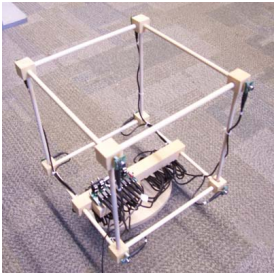
\includegraphics[width=0.75\textwidth]{./badali_2009/array.png}
\centering
\caption{The microphone array tested in \cite{badali_evaluating_2009}}
\label{fig:badali_2009_array}
\centering
\end{figure}

\begin{figure}[H]
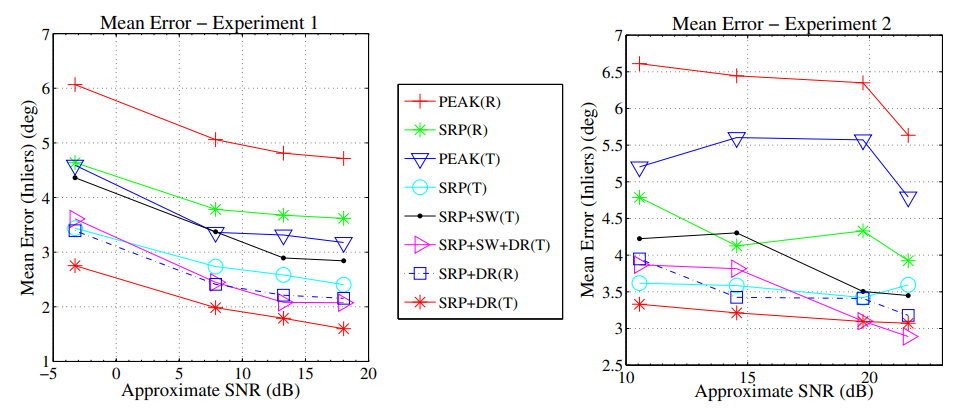
\includegraphics[width=0.75\textwidth]{./badali_2009/error_SNR.png}
\centering
\caption{The mean angular error as a function of SNR for different methods and configurations in \cite{badali_evaluating_2009}}
\label{fig:badali_2009_error_SNR}
\centering
\end{figure}

\subsubsection{Salvati et al., 2019, Power Method for Robust Diagonal Unloading Localization Beamforming}

A more recent paper \cite{salvati_power_2019} proposed diagonal unloading on a beamformer so that the system could work with high noise. This diagonal unloading was done by subtracting a diagonal matrix from the covariance matrix of the array's signal. In the robust design, the covariance matrix was estimated by the largest eigenvalue of the array's signal which was computed by the power method. This robust design was evaluated in simulation and compared against the suboptimal design using diagonal unloading, SRP-PHAT, and MUSIC. 

The array was a uniform circle of eight microphones with a radius of 20 \si{cm}, and the spatial resolution was 5 \si{\deg}. As seen in Figure-\ref{fig:salvati_2019_RMSE_SNR}, when there was a single source, the RMS error in angle of the proposed design was at most about 2.5 \si{\deg} for an SNR of at least -10 \si{dB} and grew for worse SNR. As seen in Figure-\ref{fig:salvati_2019_RMSE_SNR_two}, when there were two sources, the RMS error was at most about 4 \si{\deg} for an SNR of at least -5 \si{dB}. In all cases, the proposed robust design worked better than SRP-PHAT and suboptimal design and did just as well as MUSIC. Furthermore, despite working just as well as MUSIC, the authors claimed that their proposed design has much simpler computation of $O(M^2)$ instead of that of $O(M^3)$ where $M$ is the number of microphones.

\begin{figure}[H]
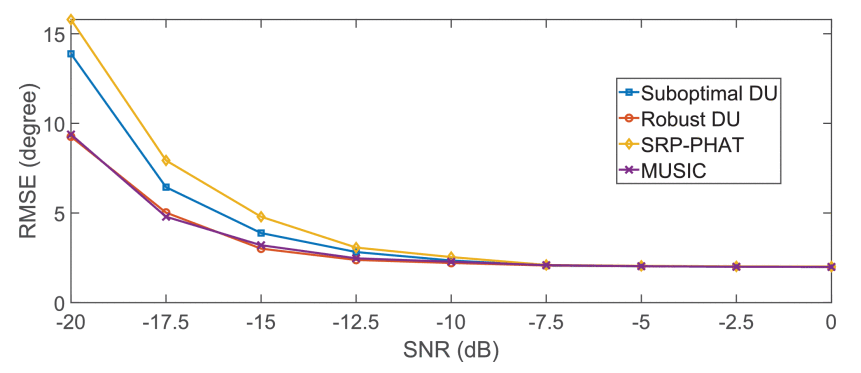
\includegraphics[width=0.75\textwidth]{./salvati_2019/RMSE_SNR.png}
\centering
\caption{The RMS error as a function of SNR for a single source in \cite{salvati_power_2019}}
\label{fig:salvati_2019_RMSE_SNR}
\centering
\end{figure}

\begin{figure}[H]
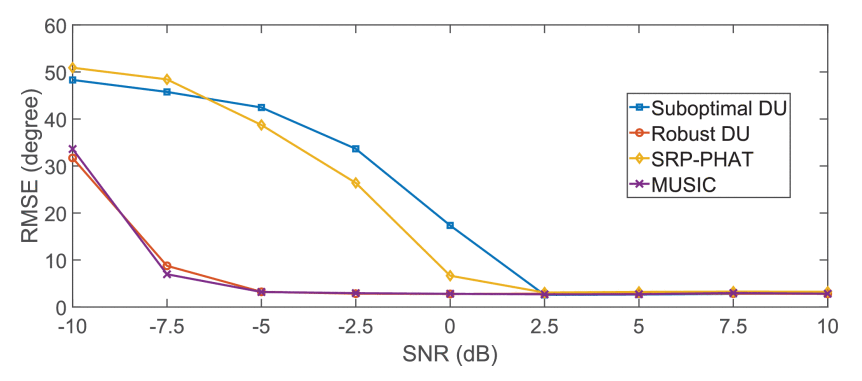
\includegraphics[width=0.75\textwidth]{./salvati_2019/RMSE_SNR_two.png}
\centering
\caption{The RMS error as a function of SNR for two sources in \cite{salvati_power_2019}}
\label{fig:salvati_2019_RMSE_SNR_two}
\centering
\end{figure}

\subsubsection{Zhang et al., 2021, An Improved Multiple Sound Source Localization Method Using a Uniform Concentric Circular Microphone Array}

The size of the array affects the beamformer. Firstly, the smaller it is, the wider the beam is especially for low frequencies. Secondly, the bigger it is, the more spatial aliasing there is, i.e. side lobes. Another recent study \cite{zhang_improved_2021} proposed a design to fix these two problems by employing an array UCCA of two concentric uniform circles of eight microphones for each. The first part of the design was frequency-classification-processing (FCP). Here, the signal's spectrum was split into bands, a lower and an upper one. A beamforming output was computed for each frequency bin. The smaller circle UCA1 used the upper band of frequencies, and the bigger circle UCA2 used the lower one. The two beamforming outputs were then summed together. The second part of the design is weighting each beamforming output; the best set of weights were found using particle-swarm-optimisation (PSO). 

The experimental array was made up a smaller circle of eight microphones with a radius of 10 \si{cm} and a bigger circle of eight with a radius of 20 \si{cm}. The experiment was done in an anechoic chamber and with two loudspeakers playing sounds of vehicle horns. Only the azimuth was tested. The proposed design worked better than the generic beamformer and had an error of 2 \si{deg} at worst as generally seen in the energy-maps in Figure-\ref{fig:zhang_2021_maps}.

\begin{figure}[H]
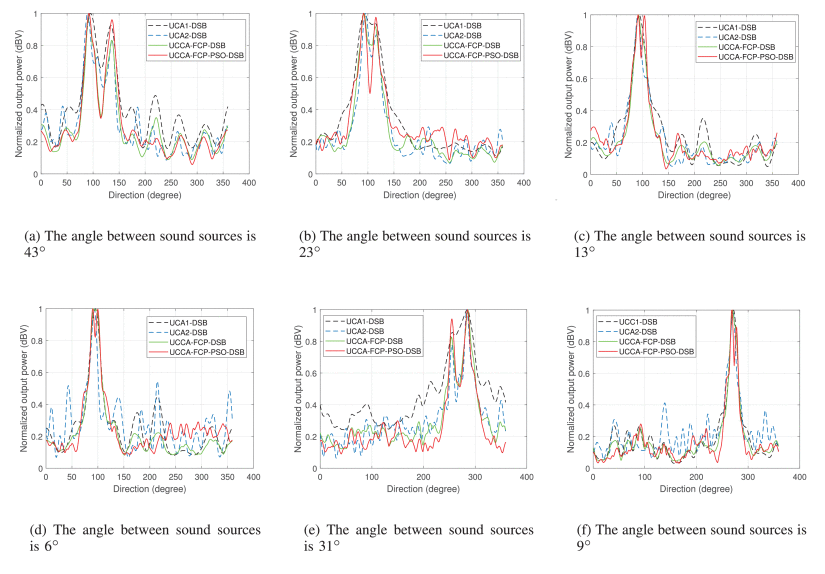
\includegraphics[width=0.75\textwidth]{./zhang_2021/maps.png}
\centering
\caption{The energy-maps of various delay-sum-beamformers (DSB) for two sources in \cite{zhang_improved_2021}}
\label{fig:zhang_2021_maps}
\centering
\end{figure}

\subsubsection{Basiri et al., 2016, On-Board Relative Bearing Estimation for Teams of Drones Using Sound}

Robotics is not the only application for localisation by beamforming. Autonomous drones are often imagined with the same capabilities of sound-source-localisation. One such study \cite{basiri_-board_2016} proposed SRP-PHAT but with a modified PHAT weighting with a power factor to mitigate the effect of noise. In order to localise multiple neighbouring drones, it also proposed a system inspired by \cite{brutti_multiple_2010} of pruning the next dominant source in the computed cross-correlation. The paper evaluated both a passive method of localising other drones' engine-sounds and an active method of localising other drones' beacons. 

The passive method which is the most relevant was tested indoors with a resting drone localising a flying drone. Motion-tracking was used to measure the true positions. The authors disclaimed that the sound of cooling fans belonging to eight tracking cameras and two computers could be heard in the room. For a single flying drone, the angular RMS error was 1.39 \si{\deg} as seen in Figure-\ref{fig:basiri_2016_histogram}. For multiple flying drones, the resting drone could localise at most three, and the precision worsen dramatically for the fourth. The array used for the passive method was a flat T-shape of four microphones seen in Figure-\ref{fig:basiri_2016_array}. The authors did not say what the exact dimension were. This study is of particular interest to robotics given that the system seemed to have been implemented on an embedded system on a drone, but the authors did not discuss computation, etc.

\begin{figure}[H]
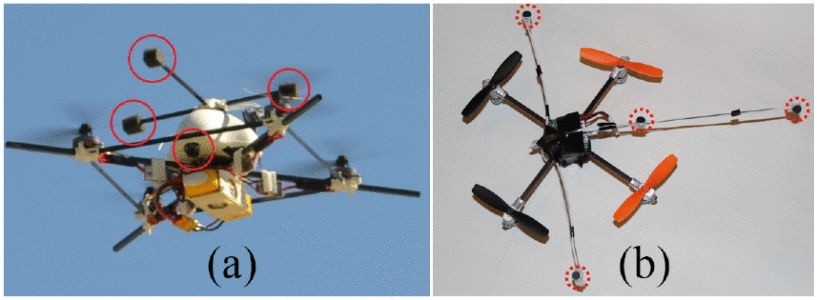
\includegraphics[width=0.75\textwidth]{./basiri_2016/array.png}
\centering
\caption{The two different microphone arrays tested in \cite{basiri_-board_2016}, namely one for the active method (a) and another for the passive method (b),}
\label{fig:basiri_2016_array}
\centering
\end{figure}

\begin{figure}[H]
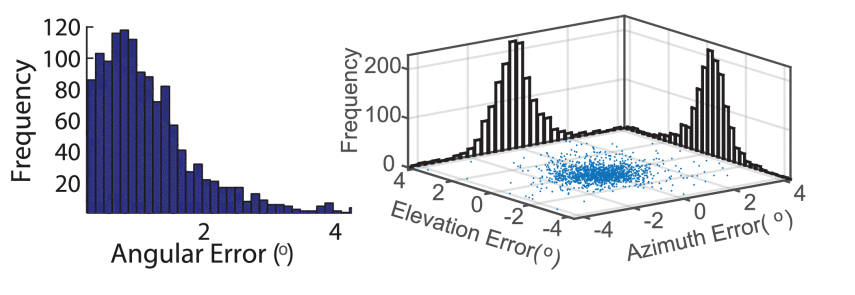
\includegraphics[width=0.75\textwidth]{./basiri_2016/histogram.png}
\centering
\caption{The histogram of the angular error for the passive method in \cite{basiri_-board_2016}}
\label{fig:basiri_2016_histogram}
\centering
\end{figure}

\subsubsection{Tamai et al., 2005, Three Ring Microphone Array for 3D Sound Localization and Separation for Mobile Robot Audition}

One paper \cite{tamai_three_2005} tested beamforming on two geometries, namely three rings of eight microphones and a larger ring of eight. The authors also proposed a method of separating sound-sources in frequency-domain, named frequency band selection (FBS), where two different directions of the beamformer are compared. However, this method works as long as the two sources do not overlap too much in the frequency-domain. Since the beam is wider at lower frequencies, a bandpass filter was applied between 1 and 3 \si{kHz}. 

In the experiments, the array of three rings was found to be more accurate than that of a single ring. The error in the azimuth of the first array was less than 3 \si{\deg} with one sound-source and less than 5 \si{\deg} with two, whilst the error in elevation was less than 6 \si{\deg} with one source. Also, the array of three rings was also able to estimate distance but only within one metre; the error of which was mostly within 300 \si{mm}.

\subsubsection{Mattos \& Grant, 2004, Passive Sonar Applications: Target Tracking and Navigation of an Autonomous Robot}

A very basic implementation for tracking only the azimuth was tested on a mobile robot \cite{mattos_passive_2004}. Here, the robot was fitted with eight microphones around it and was able to track a sound-source reliably for frequencies tested from 200 \si{Hz} to 1.2 \si{kHz}.

\section{MUSIC}

One branch of methods used to analyse and locate sound-sources separates the space of signals into subspaces. The most common kind of which is multiple-signal-classification (MUSIC). This method has a very high resolution but generally has a high computational burden, especially compared to that of TDOA or beamforming. Therefore, it is not explored as in depth as before, but the general performance across the literature is given.

The basic idea behind MUSIC is that the signals received by an array of microphones is split into subspaces, each representing either a signal or a noise. The model for the signal received is:
\begin{equation}
X = W_s S + V
\end{equation}
where 
\begin{itemize}
	\item each row of $X\in \mathbb{C}^{M\times F}$ is the received signal of the $m$-th microphone $x_m$ in the frequency-domain, i.e. $X_m$,
	\item each row of $S\in \mathbb{C}^{N\times F}$ is the $n$-th source's signal $s_n$ in the frequency-domain, i.e. $S_n$,
	\item each row of $V\in \mathbb{C}^{M\times F}$ is the noise of the $m$-th microphones in the frequency-domain,
	\item $W_s\in \mathbb{C}^{M\times S}$ is a weighting that models the time-delays of each source at each microphone for a given direction or position,
\end{itemize}
and where $M$ is the number of microphones, $F$ is the number of samples, frequency-points, etc., and $N$ is the number of sources, i.e. signals \cite{rascon_localization_2017}. The weighting is written as:
\begin{equation}
W_s[f] = 
\begin{bmatrix}
	1 						& 1						& \cdots		& 1						\\
	e^{-2\pi f\tau_{2,1}}	& e^{-2\pi f\tau_{2,2}}	& \cdots		& e^{-2\pi f\tau_{2,N}}	\\
	e^{-2\pi f\tau_{3,1}}	& e^{-2\pi f\tau_{3,2}}	& \cdots		& e^{-2\pi f\tau_{3,N}}	\\
	\vdots					& \vdots					& \ddots		& \vdots					\\
	e^{-2\pi f\tau_{M,1}}	& e^{-2\pi f\tau_{M,2}}	& \cdots		& e^{-2\pi f\tau_{M,N}}
\end{bmatrix}
\end{equation}
where $\tau_{m,n}$ is the time-delay of the $n$-th source at the $m$-th microphone.

Given this, the overall goal of MUSIC is to split the space of signals into two subspaces, namely one for signals and another for noise. This is done by eigen-decomposition of the sampled covariance matrix $R[f]\in \mathbb{C}^{N\times N}$ for a given frequency $f$.

The most basic form of MUSIC, known as standard eigen-value-decomposition (SEVD), finds the eigen-decomposition of the covariance matrix as the following:
\begin{equation}
R[f] = Q[f]\Lambda[f]Q^{-1}[f]
\end{equation}
where $\Lambda[f]$ is a diagonal matrix of the $M$ eigenvalues $\lambda_m[f]$, and each column of $Q[f]$ is a corresponding eigenvector $q_m[f]$. This matrix of eigenvectors is often split into two subspaces, $Q[f] = [Q_s[f]|Q_n[f]]$, the former for signals, and the latter for noise \cite{rascon_localization_2017}. Thereby, the spatial spectrum is found from the orthogonality between the steered direction and the eigenvectors for noise:
\begin{equation}
P(\theta_0, \phi_0)[f] = \frac{\lvert A^*(\theta_0, \phi_0) A(\theta_0, \phi_0) \rvert}
	{\sum_{m=\tilde{N}+1}^M \lvert A^*(\theta_0, \phi_0) q_m[f] \rvert}
\end{equation}
where $\tilde{N}$ is the number of sources considered, and $A(\theta_0, \phi_0)\in \mathbb{C}^{M\times 1}$ is the steering vector of transfer-functions at each microphone for a given three-dimensional direction\footnote{Much like beamforming, a full three-dimensional position can more generally be considered rather than only a direction, but again like before, this only works reliably in the near field. Since the far field is much more relevant to a small array on a robot, only direction has been considered in this example.}, i.e. an azimuth $\theta_0$ and an elevation $\phi_0$ \cite{nakamura_real-time_2012}. More simply, each row is often the lag $e^{-2\pi f\tau_m}$ where $\tau_m$ is the time-delay at the $m$-th microphone corresponding to the given direction \cite{rascon_localization_2017}.

This spatial spectrum however is narrowband for one point or bin of frequency. For a broadband response, the narrowband response is averaged over the given band of frequencies \cite{ishi_effects_2011} \cite{nakamura_real-time_2012}.

An extension of SEVD is general eigen-value-decomposition (GEVD) where the noise is whitened before the decomposition \cite{nakamura_intelligent_2009} \cite{nakamura_intelligent_2011} \cite{nakamura_real-time_2012}. Here, the eigen-decomposition is such:
\begin{equation}
K^{-1}[f] R[f] = Q[f] \Lambda[f] Q^{-1}[f]
\end{equation}
where $K[f]$ is a freely chosen matrix but is often computed as $N[f]N^*[f]$ where $N[f]$ is the frequency-domain noise recorded when there are no signals. This is shown to be more robust than SEVD for a SNR less than 0 \si{dB}.

\subsection{Literature Examples}

\subsubsection{Ishi et al., 2009, Evaluation of a MUSIC-Based Real-Time Sound Localization of Multiple Sound Sources in Real Noisy Environments}

One paper \cite{ishi_evaluation_2009} proposed a form of broadband SEVD-MUSIC where the output was the average of all the narrowband responses over a frequency-range. This was done for a small array of fourteen microphones around a robot's neck and chest as seen in Figure-\ref{fig:ishi_2009_array}. This proposed system estimated both the azimuth and the elevation on a discrete spherical grid with a resolution of about 5 \si{\deg}. Since MUSIC needs a known number of sources, the authors proposed a fixed number of sources for the narrowband MUSIC response and a maximum number of sources from the broadband response. They also compare the magnitude against a threshold to find whether the peak was a source or not. Multiple sources were nevertheless found by sequentially subtracting a two-dimensional Gaussian centred where the next highest source was; this approach is similar to others \cite{brutti_multiple_2010}, \cite{basiri_-board_2016}. 

The paper evaluated this system for a range of parameters, namely number of FFT points, frequency-range, and value of the threshold. The system was tested in a variety of "noisy environments", namely an office where the main sources of noise were an air-conditioner and the robot's hardware and an outdoor shopping mall, but the authors did not tell under what SNR and reverberation the system was tested. Nevertheless, the authors found that the system could run in real time given 64 FFT points for each frame which was about 4 \si{ms} long. Furthermore, the authors found that a frequency-range from 1 to 6 \si{kHz}, a threshold of 1.7, a fixed number of sources of 2, and a maximum number of sources of 5 were best. In most of the experiments, the accuracy was around 80 \% successful detection-rate.

\begin{figure}[H]
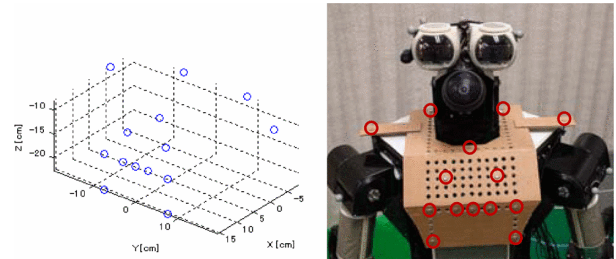
\includegraphics[width=0.75\textwidth]{./ishi_2009/array.png}
\centering
\caption{The microphone array on the robot tested in \cite{ishi_evaluation_2009}}
\label{fig:ishi_2009_array}
\centering
\end{figure}

\subsubsection{Nakamura et al., 2012, Real-Time Super-Resolution Sound Source Localization for Robots}

Another kind of MUSIC is called GEVD-MUSIC which is more robust to noise, especially the noise more powerful than the wanted signal itself. An early paper \cite{nakamura_intelligent_2009} that first proposed this kind of MUSIC in the context of robotics compared the accuracy of GEVD-MUSIC as a percentage to that of SEVD-MUSIC. The accuracy of the latter dropped below an SNR of around 5 \si{dB} whilst the accuracy of GEVD-MUSIC kept at 100 \% at an SNR of around -7 \si{dB}. In a later paper \cite{nakamura_intelligent_2011}, many of the same authors proposed the same method but with a audio-visual integration with a particle filter for tracking inactive sources and hierarchical Gaussian mixture-models. Again, the accuracy of SEVD-MUSIC dropped at an SNR of around -8 \si{dB}, whilst that of GEVD-MUSIC dropped at an SNR of around -14 \si{dB}. 

To ease the computation, the same authors proposed a new kind of MUSIC called GSVD-MUSIC \cite{nakamura_real-time_2012}. To further lessen computation, the authors proposed a hierarchical search from coarse to fine, and to improve the resolution, they linearly interpolated the transfer-functions in both the frequency- and time-domain. The accuracy of the proposed GSVD-MUSIC only began to drop at an SNR fo around -10 \si{dB}, about 5 \si{dB} less than that of GEVD-MUSIC. The average error in the azimuth was at best about 1 \si{\deg} and at worst about 10 \si{\deg}. The proposed method also worked well for a moving source. The array was a circle of eight microphones embedded in the robot's head. The authors claimed that their new method of GSVD-MUSIC lessened the computational cost by 40.6 \% compared to GEVD-MUSIC and that their design of a hierarchical search lessened it by a further 59.2 \% for a single source. However, the computation was done on a laptop, and no comparison was made with other methods of sound-source-localisation such as SRP-PHAT.
% discussion: array on head

\begin{figure}[H]
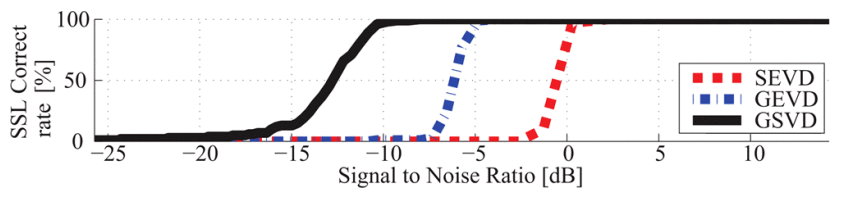
\includegraphics[width=0.75\textwidth]{./nakamura_2012/rate_SNR.png}
\centering
\caption{The rate of successful localisations against SNR for SEVD, GEVD, and the proposed GSVD in \cite{nakamura_real-time_2012}}
\label{fig:nakamura_2012_rate_SNR}
\centering
\end{figure}

\section{Discussion of the Literature}

Many examples and methods in the literature have been discussed. Here, a summary of the most relevant examples is given. The following attributes are compared:
\begin{itemize}
	\item the type of method, i.e. one of three categories discussed so far, namely TDOA, beamforming, and MUSIC,
	\item the specific method itself,
	\item the result or output of the algorithm, i.e. the type of localisation whether it is the direction only or the full three-dimensional coordinates (note that some methods could estimate distance but only in the near field; here, only the result in the far field is considered),
	\item the number of sources detectable, often either single or multiple,
	\item the accuracy or precision,
	\item the built-in resolution of the method,
	\item the number of microphones in the array,
	\item the array's dimensions (given a complex array, only the widest displacement is given),
	\item the distances tested,
	\item the noise under which the method was tested or for which it is rated, often given as the SNR,
	\item the reverberation under which the method was tested,
	\item the sampling rate,
	\item the length of the frame, window, or block of samples (may be in either number of samples or simply time),
	\item any comments on the computation, e.g. whether the method runs in real-time, what the method was computed on, etc.,
	\item and any comments about the design or method.
\end{itemize}

\subsection{Accuracy and Estimation}

Nearly all methods only compute the three-dimensional angle. Only two attempt full three-dimensional position, i.e. direction along with distance. However, only Chen \& Xu in 2019 \cite{chen_sound_2019} seemed to attempt this in the far field for distances more than 1 \si{m}; Bechler et al. in 2004 \cite{bechler_system_2004} only have tested within about 1 \si{m} which may considered to be the near field given the dimensions of their array.

A common theme throughout the literature-review is the inconsistent calculation of accuracy. Some papers used the RMS error (RMSE), the mean-squared error (MSE), or simply the average error itself. Some papers did not even give error but rather the percentage of successful localisation relative to the resolution. Furthermore, it is hard to summarise the accuracy of a method given that it varies depending on noise, distance, etc. Here, the accuracy at best and at worst is given as lower and upper bounds. Nonetheless, most methods tended to have an error of 2 \si{\deg}.

\subsection{Dimensions}

Although some dimensions were not given at all, e.g. Basiri et al. in 2016 \cite{basiri_-board_2016}, the smallest array seemed to be that of Hu et al. in 2009 \cite{hu_estimation_2009}. The biggest was that of Valin et al. in 2003 and 2004 (both papers use the same array but different methods) \cite{valin_robust_2003} \cite{valin_localization_2004}.

\subsection{Noise and Reverberation}

As for noise, Manamperi et al. in 2022 \cite{manamperi_drone_2022} tested up to the worst SNR of -30 \si{dB} although this paper was specifically about mitigating noise in the context of drones. Whilst for reverberation, Bechler et al. in 2004 \cite{bechler_system_2004} had the longest reverberation-time of 0.36 \si{ms} at 60 \si{dB}. Again however, many papers neglect any information about noise or reverberation, some albeit with vague descriptions.

\subsection{Computation}

Most methods could run in real-time albeit on laptop and desktop computers. However, Basiri et al. in 2016 \cite{basiri_-board_2016} seemed to be the only example implemented on an embedded system on the drone itself, namely an Atmel AVR32 microcontroller. This example is therefore of particular interest to this project given the want for an embedded implementation.

% closed array

% noise-mitigation

% notable authors

\chapter{Simulation}

\section{Software}

\subsection{Python}

Most of the simulation had been done in Python which is a free and popular programming language that has many free and open-source third-party libraries to help simulate physical and mathematical phenomena. It also has many tools to help plot data and concepts.

Some Python modules used are:
\begin{itemize}
	\item numpy,
	\item scipy,
	\item matplotlib,
	\item and pyroomacoustics.
\end{itemize}

\subsection{Pyroomacoustics}

One very important aspect of the simulation was to emulate the effect of a room on the sound recorded by a microphone. This is commonly taken as the reverberation or more specifically the reverberation-impulse-response (RIR) which can be used to compute the sound recorded by convolution on the original.

A very helpful Python module was that called Pyroomacoustics which was made specifically for simulating arrays of microphones. It could compute the RIR given the dimensions of a room, the location of the source, the location of the microphone, and other parameters such as the absorption-factor of the walls. The module mainly uses the image-source model (ISM) which is a common model for reverberation as well as optionally ray-tracing. It could also simulate with an array of microphones and superpose noise on the signal.

It also had a suite of functions and examples for sound-source-localisation, but these were mostly ignored since the purpose of the simulations was to recreate existing examples in the literature and to study the methods from first principles.

\subsection{Sounds}

For sounds, a variety of sounds were taken from \textit{freesound.org} which has a corpus of free and public recordings of sounds mostly under the Attribution 4.0 licence \footnote{https://creativecommons.org/licenses/by/4.0/}.

\section{Evaluation of Examples in the Literature}

In order to choose the best method for this project, some of the examples in the literature must be evaluated in the simulation first, especially against the effects of noise and reverberation. So far, only two examples were studied, namely:
\begin{itemize}
	\item the TDOA-based and iteration-based method used on a rectangular pyramid array that can estimate the distance as well as the direction \cite{chen_sound_2019}
	\item and the common SRP-PHAT method used for beamforming \cite{valin_localization_2004} \cite{valin_robust_2007}.
\end{itemize}


%\subsection{Analysis of GCC-PHAT}

\subsection{Rectangular Pyramid Array with TDOA}

One example in the literature that stands out is the paper describing an array as a rectangular pyramid on a mobile robot \cite{chen_sound_2019} since it is one of the few examples that claim to estimate distance as well as direction. The estimation of distance is a highly valuable ability in this project. Therefore, it was the first example to evaluate.

\subsubsection{Algorithm}

As said before, the array was a rectangular pyramid 0.25 \si{m} wide and 0.125 \si{m} tall as seen in Figure-\ref{fig:chen_2019_array}. The algorithm described in the paper \cite{chen_sound_2019} was seemingly complex. It worked on one frame of signals, i.e. a block of samples representing a duration of time. Each frame was made up of multiple channels for each microphone, in this case, five channels. 

Firstly, the TDOA was estimated for each pair, or permutation, of microphones. The matrix of which was averaged diagonally in magnitude only since there was some redundancy in mirrored TDOAs, i.e. $\Delta t_{ij} = -\Delta t_{ji}$. Since the algorithm used an iterative approach, it needed an initial guess. The paper described albeit vaguely a strategy of comparing TDOAs of adjacent pairs. This would break the space up into eight sectors or partitions seen in Figure-\ref{fig:chen_2019_partitions}, in one of which the source lied. Given a lack of detail, this was interpreted as in Algorithm-\ref{alg:pyramid_guess}.

\begin{figure}[H]
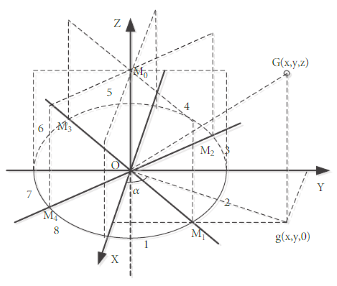
\includegraphics[width=1\textwidth]{./chen_2019/partitions.png}
\centering
\caption{The partitions in space of the rectangular pyramid array are used such that an initial condition can be guessed and fed to the iterative algorithm \cite{chen_sound_2019}.}
\label{fig:chen_2019_partitions}
\centering
\end{figure}

\begin{algorithm}[H]
\caption{Guessing the general direction from a rectangular pyramid}
\label{alg:pyramid_guess}
\begin{algorithmic}
	\For{every $i$-th microphone on the corners of the pyramid's base}
		\State $a \gets$ the index of the left adjacent microphone
		\State $b \gets$ the index of the right adjacent microphone
		\For{$j = a, b$}
			\State Get the TDOA as $\Delta t_{ji}$
		\EndFor
		\If{$\Delta t_{ai} > 0$ \textbf{ and } $\Delta t_{bi} > 0$}
			\If{$\Delta t_{ai} > \Delta t_{bi}$}
				\State $k \gets a$
			\Else
				\State $k \gets b$
			\EndIf
			\State $r_i$ is the position of the $i$-th microphone.
			\State $r_k$ is the position of the $k$-th microphone.
			\Comment{The source lies between the sector spanned by the $i$-th microphone and the $k$-th microphone.}
			\State $r \gets 2 (r_{i} + r_{k})$ \Comment{Make a vector that lies within this sector.}
		\EndIf
	\EndFor
\end{algorithmic}
\end{algorithm}

Next, the paper laid out a strategy of calculating four estimates given that only three TDOAs were needed for the iterative algorithm. Here, the top microphone has an index of 0, whilst the others have indices of 1, 2, 3, and 4. Thus, given three TDOAs $\Delta t_{0j}$, the position of the source could be found by the following model:
\begin{equation}
\begin{split}
f_j(x,y,z) &= \sqrt{\left(x-x_j\right)^2 + (y - y_j)^2 + (z - z_j)^2} \\
&- \sqrt{\left(x-x_0\right)^2 + (y - y_0)^2 + (z - z_0)^2}
- c \Delta t_{j0}
\end{split}
\end{equation}
where $j = 1, 2, 3, 4$, and $c$ is the speed of sound.

This was solved by the iterative formula based on Newton's well known method.
\begin{equation}
\begin{bmatrix}
	x^{(k+1)} \\
	y^{(k+1)} \\
	z^{(k+1)}
\end{bmatrix}
=
\begin{bmatrix}
	x^{(k)} \\
	y^{(k)} \\
	z^{(k)}
\end{bmatrix}
-
J^{-1}
\begin{bmatrix}
	f_1\left(x^{(k)}, y^{(k)}, z^{(k)}\right) \\
	f_2\left(x^{(k)}, y^{(k)}, z^{(k)}\right) \\
	f_3\left(x^{(k)}, y^{(k)}, z^{(k)}\right)
\end{bmatrix}
\end{equation}
where $J$ is the Jacobian as such:
\begin{equation}
J = 
\begin{bmatrix}
\frac{\partial f_1}{\partial x}
& \frac{\partial f_1}{\partial y}
& \frac{\partial f_1}{\partial z} \\
\frac{\partial f_2}{\partial x}
& \frac{\partial f_2}{\partial y}
& \frac{\partial f_2}{\partial z} \\
\frac{\partial f_3}{\partial x}
& \frac{\partial f_3}{\partial y}
& \frac{\partial f_3}{\partial z}
\end{bmatrix}
\end{equation}

The paper did not give a maximum number of iterations, but in this study, at most a hundred were tried since the algorithm seemed to find the solution within twenty iterations. Sometimes however, depending on the initial condition, the algorithm would diverge rapidly which would eventually lead to a singular matrix. In the Python simulation, a condition was checked whether the estimated position was further than 100 \si{m} from the array; in which case, it could be safely assumed that the iterative algorithm had failed which was then aborted. This would be counted and logged as a failure.

Since the iterative algorithm only needed three TDOAs from three pairs of the top microphone with the three corner microphones, four estimates could be gotten. These were then averaged to give the final estimated position of the source.

\subsubsection{Experimental Method}

The microphone-array was set 1 \si{m} off the floor in the centre of a closed room 10 \si{m} wide, 10 \si{m} long, and 3 \si{m} high. The rectangular base of the array was also oriented to be in line with the room. Given that the origin was in one bottom corner of the room, the coordinates of the centre of the array's rectangular base were $(5,5,1)$. Furthermore, an absorption factor of 0.5 was used for the walls. This gave RIRs as seen in Figure-\ref{fig:pyramid_robot_noise_rir} and an estimated reverberation-time at 60 \si{dB} of 84.8 \si{ms}. This would roughly emulate a large indoor office-space with moderate reverberation.

\begin{figure}[H]
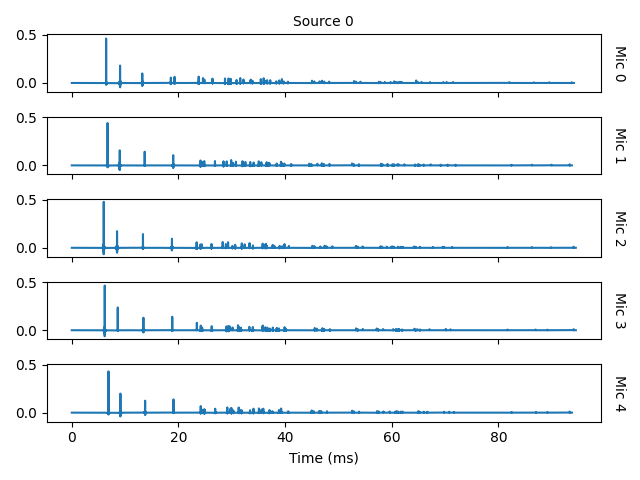
\includegraphics[width=1\textwidth]{../Python/pyramid_robot/noise/rir.png}
\centering
\caption{An example of the RIR made from the Pyroomacoustics module is shown.}
\label{fig:pyramid_robot_noise_rir}
\centering
\end{figure}

For the sound, a recording of claps taken in an anechoic chamber was used \cite{noauthor_handclaps_2005}. After it was simulated in the room-environment, a single frame of 8192 samples was analysed in the algorithm.

\subsubsection{Performance against Noise}

The first experiment was to evaluate the performance against noise, specifically additive Gaussian white noise (AGWN). Overall, ten levels of noise were simulated for which, i.e. SNRs from -20 to 25 \si{dB}. For each level of noise, ten thousand runs of the simulation were done in order to calculate the mean and variance of the estimated values. Thereby, the accuracy of the method was given by how much the mean deviates from the true value, and the precision and repeatability were given by how much the variance increases.

The source was fixed with the coordinates of $(5.5,3,1)$ as seen in Figure-\ref{fig:pyramid_robot_room_3d} and -\ref{fig:pyramid_robot_room_2d}. This makes the source 2.06 \si{m} away from the centre of the array with an azimuth of 76.0 \si{\deg} and with an elevation of 90 \si{\deg}.

\begin{figure}[H]
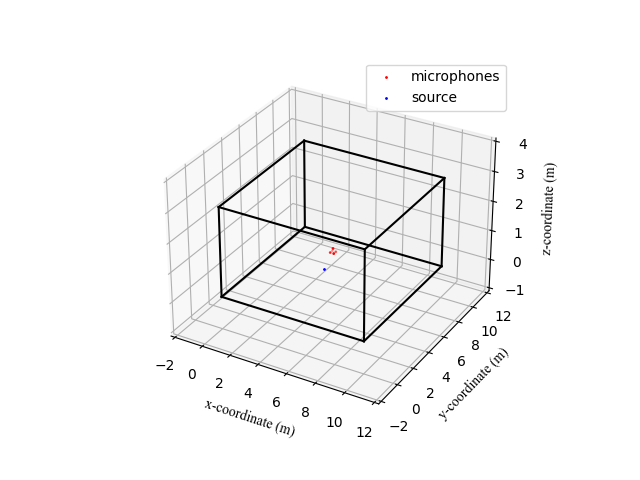
\includegraphics[width=1\textwidth]{../Python/pyramid_robot/room_3d.png}
\centering
\caption{The 3D room is shown and has the rectangular pyramid array in the centre 1 \si{m} off the ground and with the source at $(5.5,3,1)$.}
\label{fig:pyramid_robot_room_3d}
\centering
\end{figure}

\begin{figure}[H]
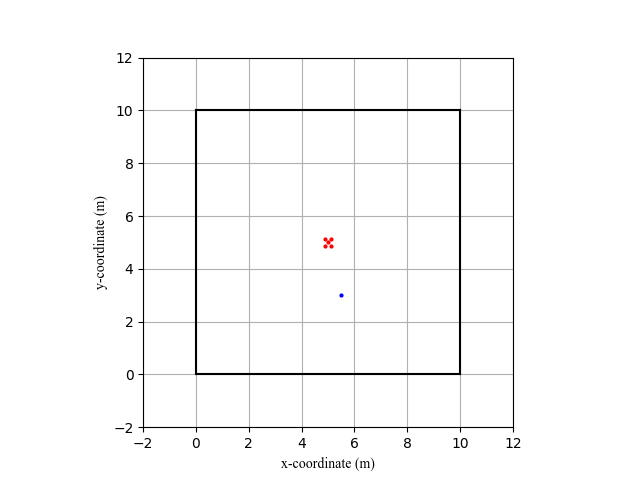
\includegraphics[width=1\textwidth]{../Python/pyramid_robot/room_2d.png}
\centering
\caption{A bird's-eye-view of the room is shown with the rectangular pyramid array in the centre 1 \si{m} off the ground and with the source at $(5.5,3,1)$.}
\label{fig:pyramid_robot_room_2d}
\centering
\end{figure}

The performances for the estimated distance, the estimated azimuth, and the estimated elevation are given in Figure-\ref{fig:pyramid_robot_noise_distance}, -\ref{fig:pyramid_robot_noise_azimuth}, and -\ref{fig:pyramid_robot_noise_elevation} respectively.

% Fix the y-axis labels.

\begin{figure}[H]
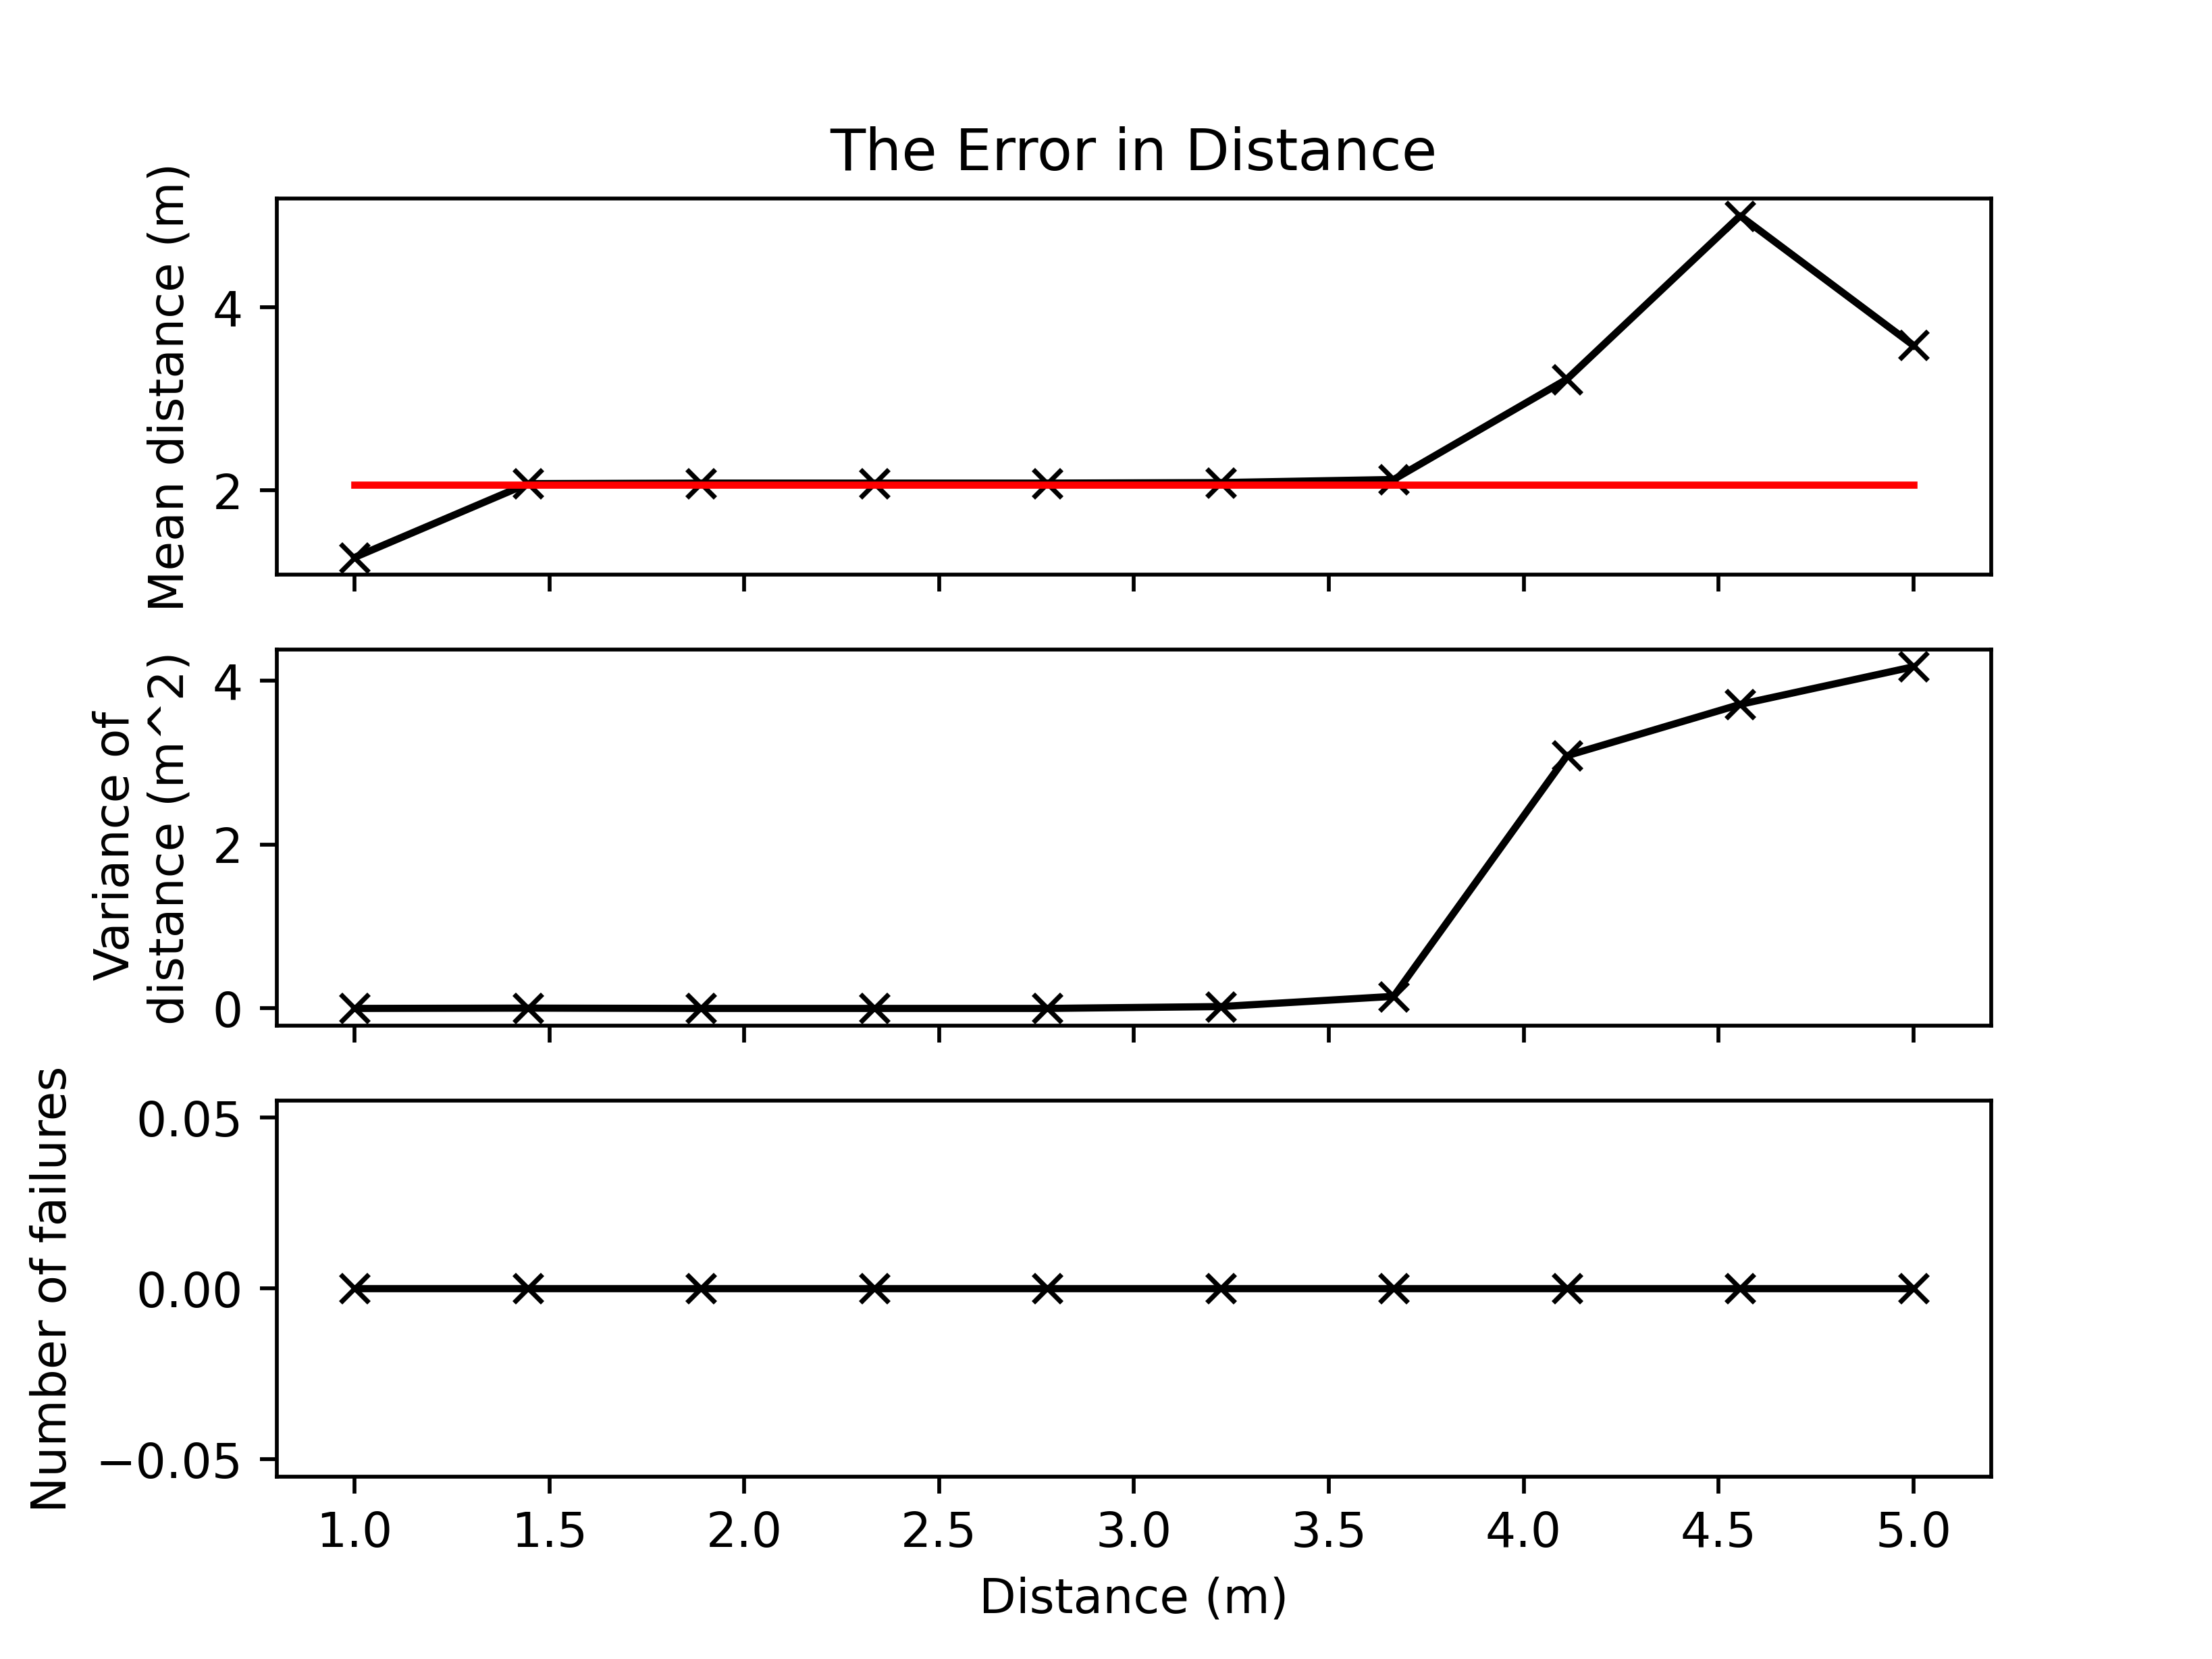
\includegraphics[width=1\textwidth]{../Python/pyramid_robot/noise/distance.png}
\centering
\caption{The statistical performance of estimated distance is plotted against noise; the red line is the true distance.}
\label{fig:pyramid_robot_noise_distance}
\centering
\end{figure}

\begin{figure}[H]
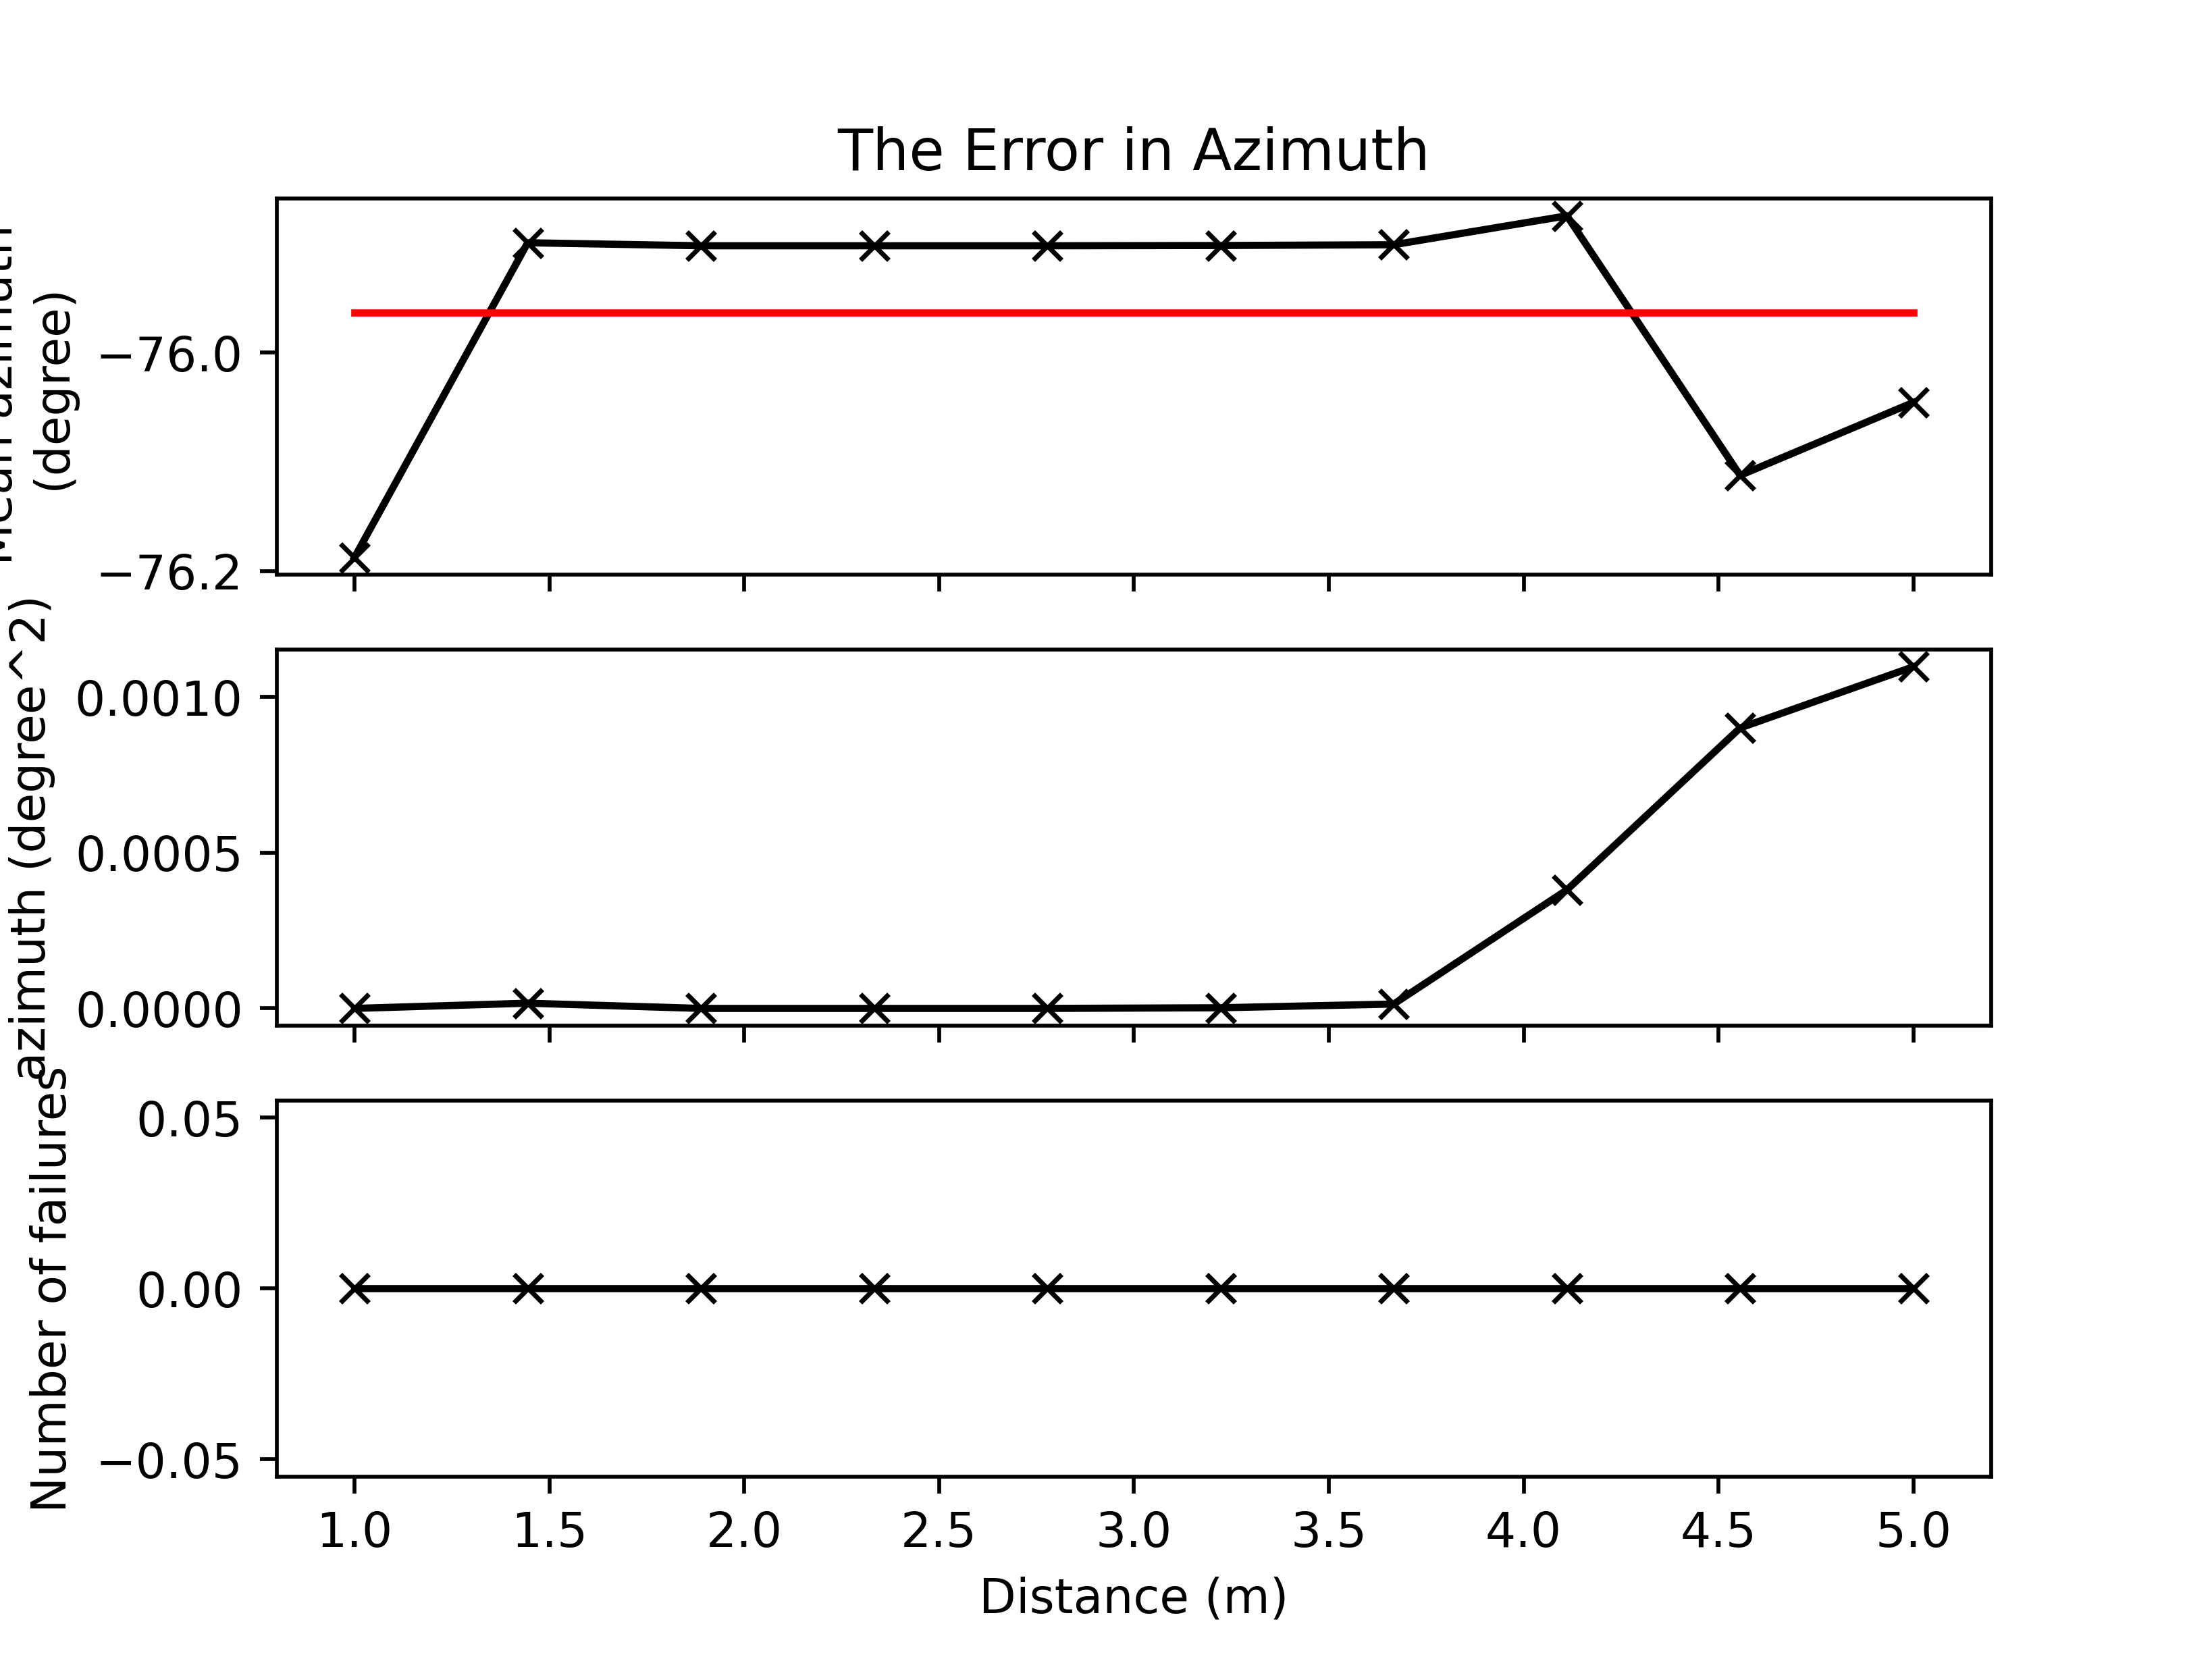
\includegraphics[width=1\textwidth]{../Python/pyramid_robot/noise/azimuth.png}
\centering
\caption{The statistical performance of estimated azimuth is plotted against noise; the red line is the true azimuth.}
\label{fig:pyramid_robot_noise_azimuth}
\centering
\end{figure}

\begin{figure}[H]
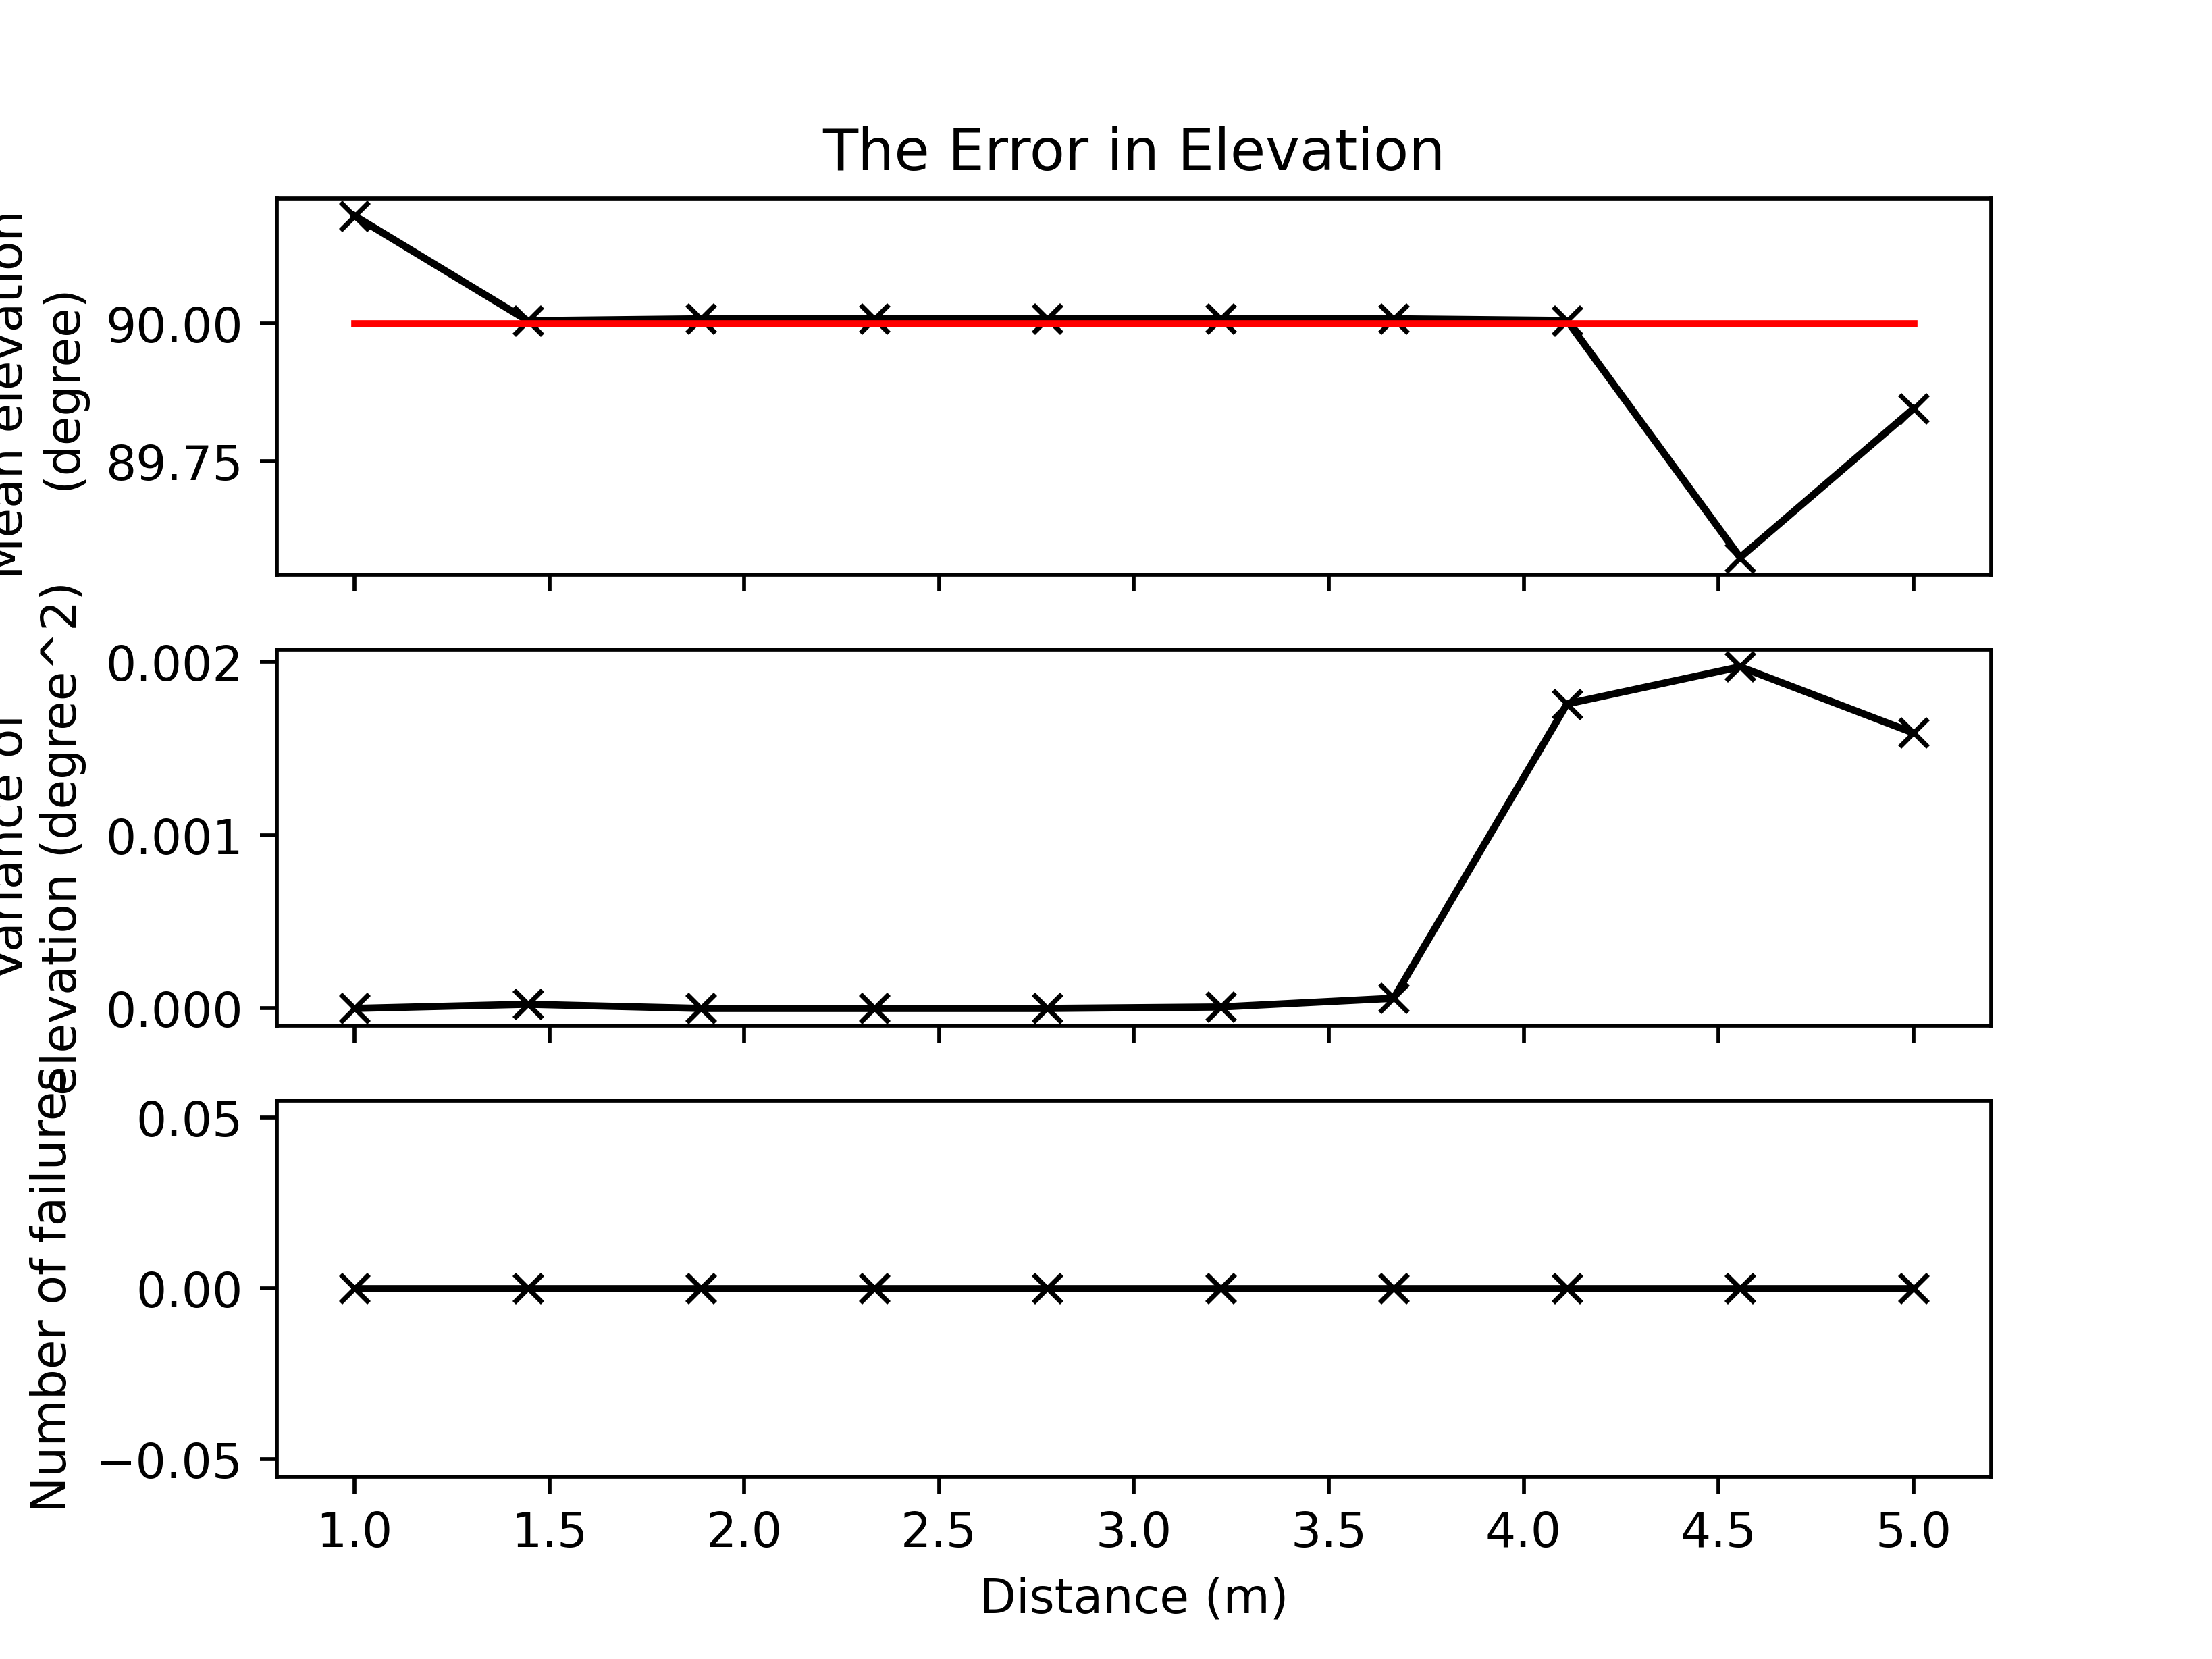
\includegraphics[width=1\textwidth]{../Python/pyramid_robot/noise/elevation.png}
\centering
\caption{The statistical performance of estimated elevation is plotted against noise; the red line is the true elevation.}
\label{fig:pyramid_robot_noise_elevation}
\centering
\end{figure}

From these results, the estimated direction, i.e. both the azimuth and the elevation, had very little variance and little bias which albeit became worse with noise. However, the estimated distance was worsened much more as seen in Figure-\ref{fig:pyramid_robot_noise_distance} with high bias and variance. Furthermore, the number of failures in the iterative algorithm became significantly worse as noise was increased. This in fact made the calculation of the mean and the variance for all three values hard since it no longer followed the law of large numbers. This may explain the odd values for the mean and the variance for the first few noise-levels, i.e. towards the left of the plot.

\subsubsection{Performance against Distance}

The next experiment was to evaluate the performance against distance. Overall, ten levels of noise were simulated for which, i.e. SNRs from -20 to 25 \si{dB}. For each level of noise, ten thousand runs of the simulation were done in order to calculate the mean and variance of the estimated values. Thereby, the accuracy of the method was given by how much the mean deviates from the true value, and the precision and repeatability were given by how much the variance increases.

The source was fixed with the coordinates of $(5.5,3,1)$ as seen in Figure-\ref{fig:pyramid_robot_room_3d} and -\ref{fig:pyramid_robot_room_2d}. This makes the source 2.06 \si{m} away from the centre of the array with an azimuth of 76.0 \si{\deg} and with an elevation of 90 \si{\deg}.

\subsubsection{Discussion}

Although it was one of the few that estimates the distance, this method relies on an iterative algorithm and thus relies on an initial condition. It was found in simulation that this iterative algorithm was highly sensitive to inaccurate estimations of the TDOAs. This would often lead to the iterative algorithm failing to converge. This would especially happen if the noise was high which would lead to peaks at zero in the GCC-PHAT and this would give an inaccurate TDOA. This can be clearly seen as the number of failures grew as the noise was increased in Figure-\ref{fig:pyramid_robot_noise_distance}. The iterative algorithm was also found to be sensitive to the choice of the initial condition.

\subsection{SRP-PHAT}

This section will study a common method of beamforming shared among a few papers reviewed so far, namely SRP-PHAT. In particular, it was used on mobile robots \cite{valin_localization_2004}, \cite{valin_robust_2007}.

\subsubsection{Algorithm}

In this simulation, a modified PHAT spectral weighting was used as described in \cite{valin_localization_2004}, and similar to that in \cite{valin_robust_2003}:
\begin{equation}
\psi_{m_i,m_j}(\tau) = \frac{1}{\lvert X_{m_i}(k) \rvert \lvert X_{m_j}(k) \rvert}
\end{equation}
The special weighting is:
\begin{equation}
w(k) =
\begin{cases}
	1,										& Y(k) \leq Y_N(k) \\
	\left( \frac{Y(k)}{Y_N(k)}\right)^\gamma	& Y(k) > Y_N(k)
\end{cases}
\end{equation}
where $\gamma$ is set as 0.1\footnote{This was chosen from \cite{valin_localization_2004} but can be easily tuned if need be.}, $Y(k)$ is the mean spectral density across all microphones, and $Y_N(k)$ is the noise estimate as the average of $Y(k)$ across time. Here, neither paper went into much depth about the calculation of $Y_N(k)$; so, it was assumed that it was the average for all runtime instead of a moving window. This modified weighting would weight frequencies with higher SNR more to lessen the effect of noise and also to better the detection of narrowband signals.

As seen in Figure-\ref{fig:srp_phat_grid}, a spherical grid of 2562 points was used as a search-grid of directions as described in some of the papers \cite{valin_localization_2004} \cite{valin_robust_2007}. This was generated by tessellating an icosahedron.

\begin{figure}[H]
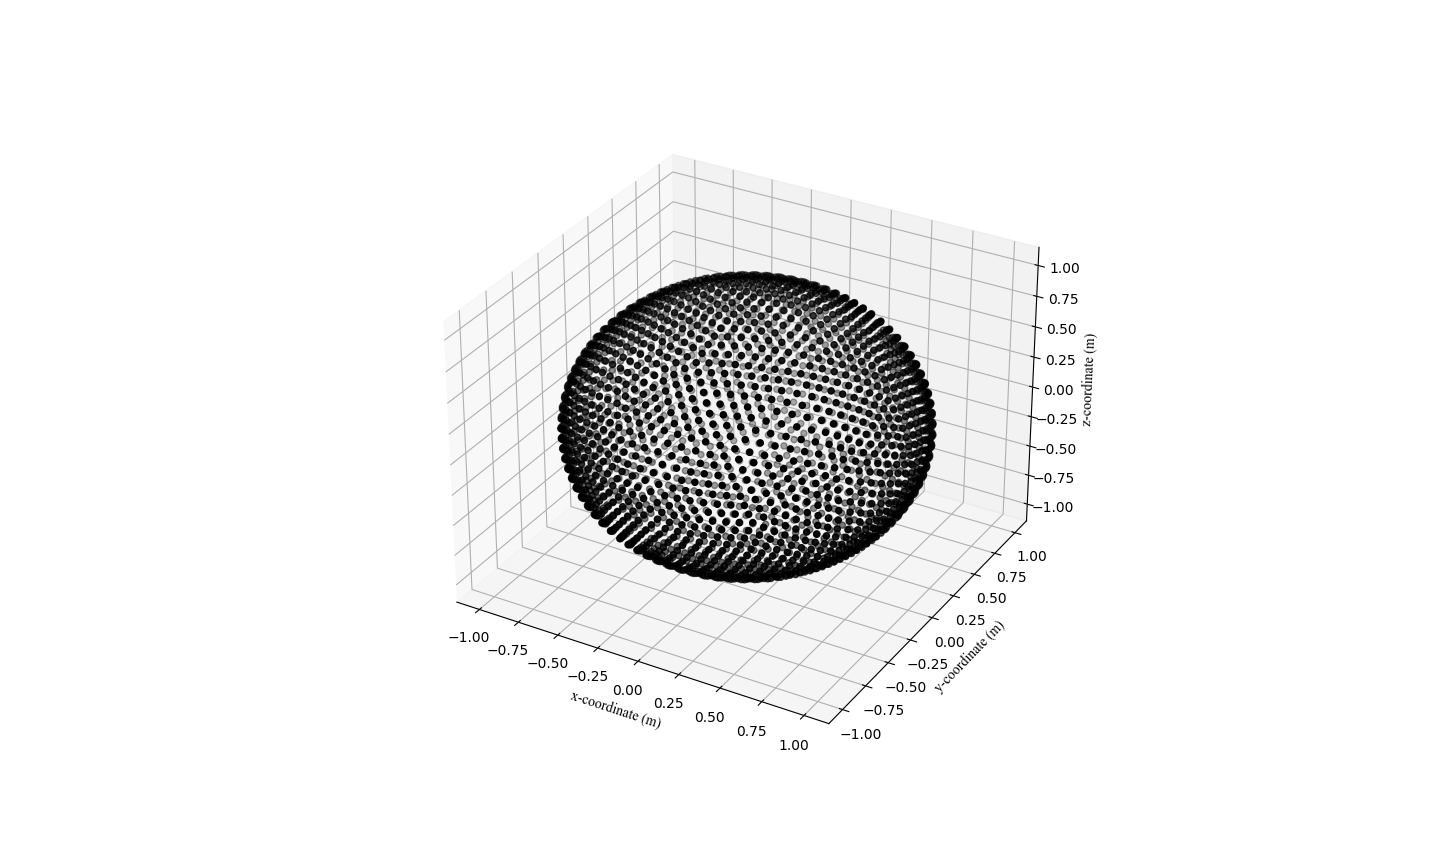
\includegraphics[width=1\textwidth]{../Python/srp_phat/grid.png}
\centering
\caption{The spherical grid of directions was used to estimate the direction of the sound-source using SRP-PHAT.}
\label{fig:srp_phat_grid}
\centering
\end{figure}

Each of these points was used as a direction along which to steer the beamformer and thus to draw a spherical energy-map. The direction that corresponded to the highest energy was the estimated direction of the source.

\subsubsection{Experimental Method}

The dimensions of the tested microphone-array were taken from one of the often cited papers for the SRP-PHAT \cite{valin_robust_2007}, namely a cube 15.5 \si{cm} wide. The array was set up the same way as before; that is 1 \si{m} off the floor in the centre of a closed room 10 \si{m} wide, 10 \si{m} long, and 3 \si{m} high. The array was also oriented to be in line with the room. Given that the origin was in one bottom corner of the room, the coordinates of the array's centre were $(5,5,1)$. Furthermore, an absorption factor of 0.5 was used for the walls. This gave RIRs as seen in Figure-\ref{fig:pyramid_robot_rir} and an estimated reverberation-time at 60 \si{dB} of 84.8 \si{ms}. This would roughly emulate a large indoor office-space with moderate reverberation.

For the sound, two kinds were tested; first, a recording of claps taken in an anechoic chamber was used \cite{noauthor_handclaps_2005}; secondly, a recording of a whistle. The former sound models a typical broadband signal, whilst the latter models a typical narrowband signal. These sounds were resampled to 48 \si{kHz} to ensure a consistent analysis.

After it was simulated in the room-environment, a single frame of 1024 samples was analysed in the algorithm, but all other frames before that were analysed to calculate the noise spectral density.

\subsubsection{Stastical Performance against Noise}

The first experiment was to evaluate the performance against noise, specifically additive Gaussian white noise (AGWN). Overall, ten levels of noise were simulated for which, i.e. SNRs from -20 to 25 \si{dB}. Ten thousand runs of the simulation for each noise-level were done in order to calculate the mean and variance of the estimated values. Thereby, the accuracy and the bias of the method was given by how much the mean deviates from the true value, and the precision and repeatability were given by how much the variance increases.

The source was fixed with the coordinates of $(5.5,3,1)$  as seen in Figure-\ref{fig:srp_phat_room_3d} and -\ref{fig:srp_phat_room_2d}. This makes the source 2.06 \si{m} away from the centre of the array with an azimuth of 76.0 \si{\deg} and with an elevation of 90 \si{\deg}.

\begin{figure}[H]
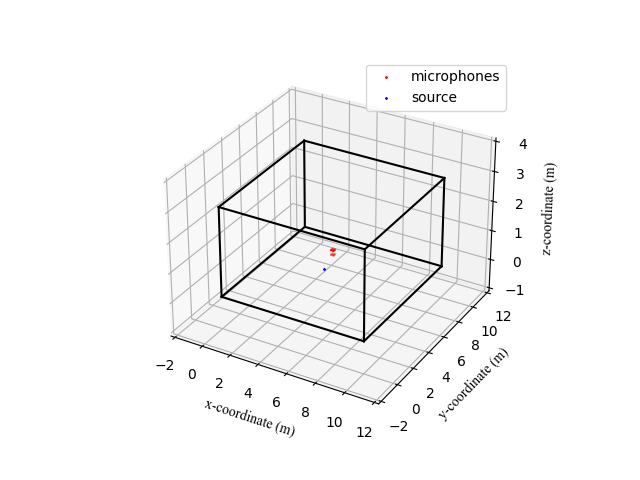
\includegraphics[width=1\textwidth]{../Python/srp_phat/room_3d.png}
\centering
\caption{The 3D room is shown and has the cubic array for testing the SRP-PHAT method in the centre 1 \si{m} off the ground and with the source at $(5.5,3,1)$.}
\label{fig:srp_phat_room_3d}
\centering
\end{figure}

\begin{figure}[H]
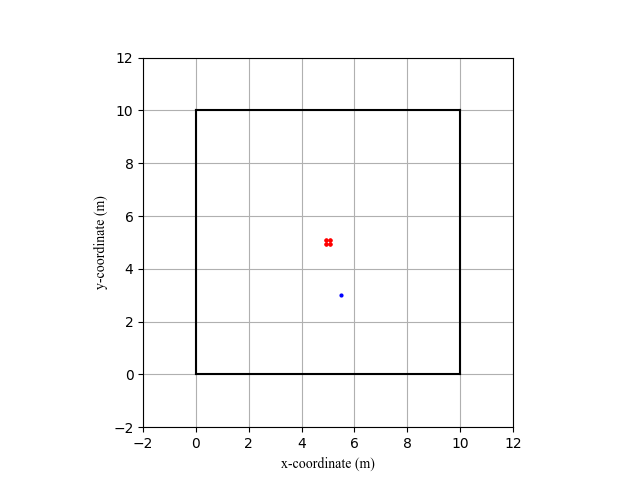
\includegraphics[width=1\textwidth]{../Python/srp_phat/room_2d.png}
\centering
\caption{A bird's-eye-view of the room is shown with the cubic array for testing the SRP-PHAT method in the centre 1 \si{m} off the ground and with the source at $(5.5,3,1)$.}
\label{fig:srp_phat_room_2d}
\centering
\end{figure}

The performances for the estimated azimuth and the estimated elevation are given in Figure-\ref{fig:srp_phat_noise_clap} and -\ref{fig:srp_phat_noise_whistle} respectively.

\begin{figure}[H]
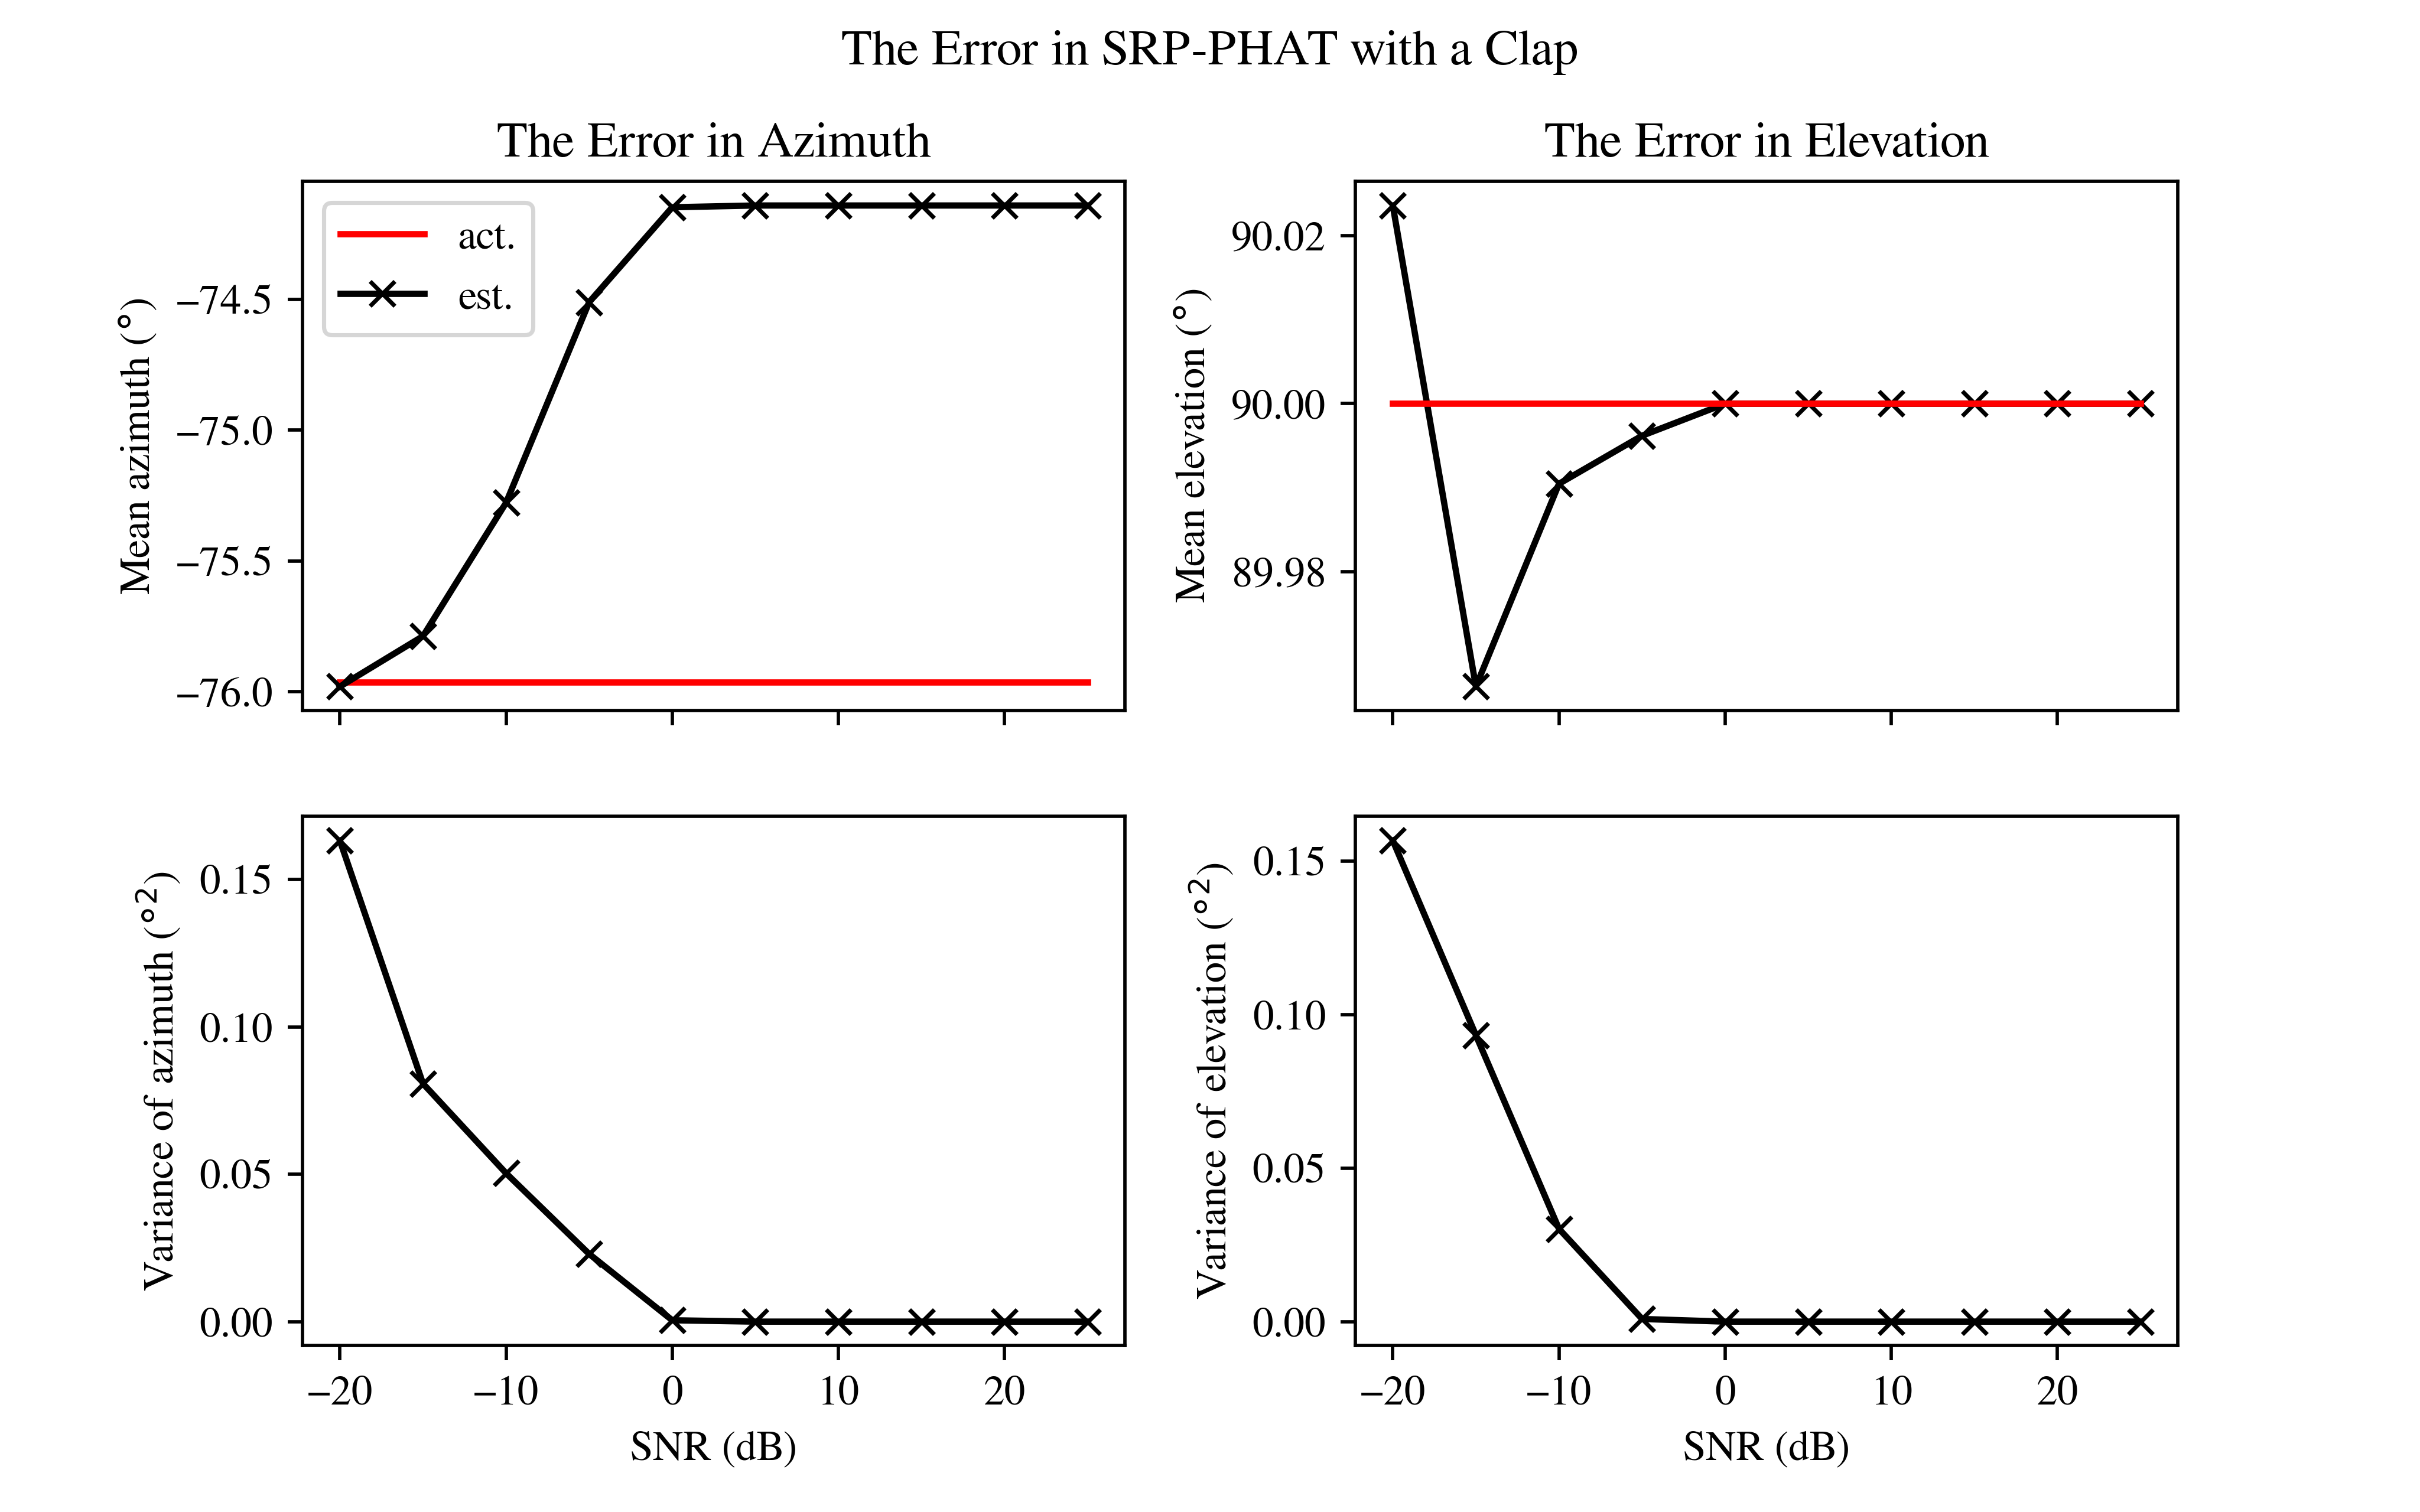
\includegraphics[width=1\textwidth]{../Python/srp_phat/noise/clap/plots.png}
\centering
\caption{The statistical performance of the estimated direction is plotted against noise with a clap as the source.}
\label{fig:srp_phat_noise_clap}
\centering
\end{figure}

\begin{figure}[H]
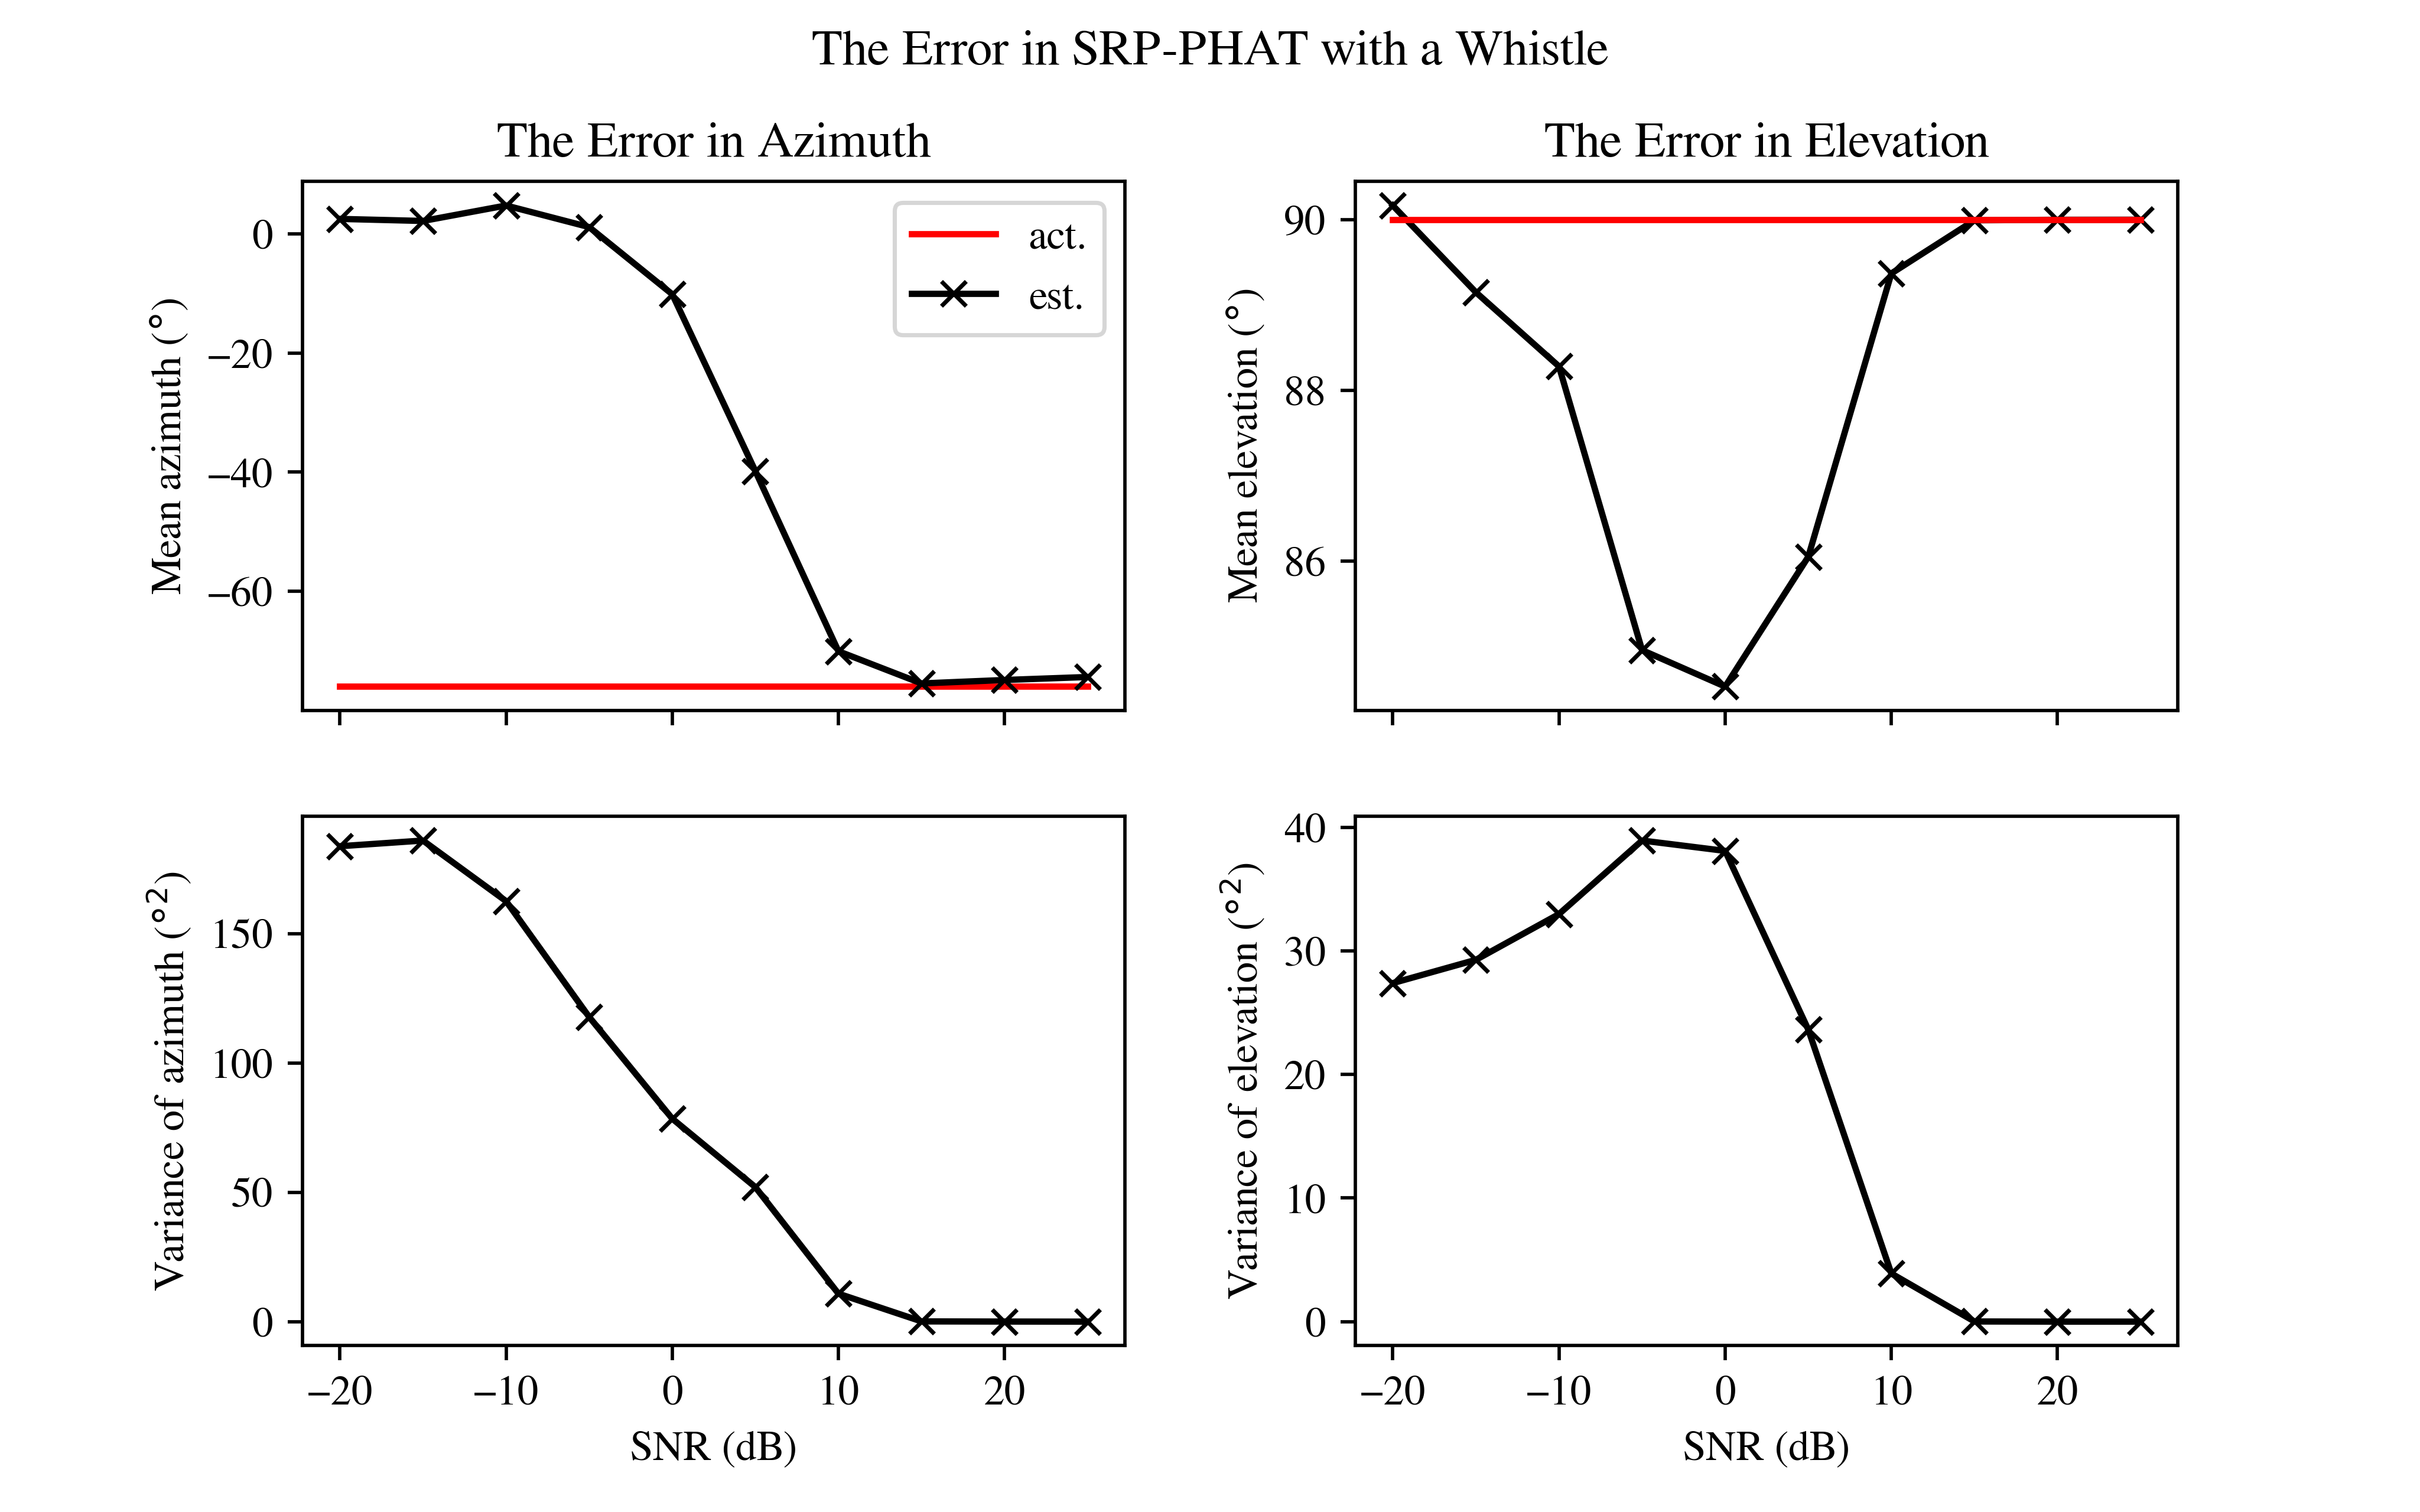
\includegraphics[width=1\textwidth]{../Python/srp_phat/noise/whistle/plots.png}
\centering
\caption{The statistical performance of the estimated direction is plotted against noise with a whistle as the source.}
\label{fig:srp_phat_noise_whistle}
\centering
\end{figure}

With a broadband signal like a clap, it was seen from these results that the method was fairly robust against noise since there is very little variance in both the estimated azimuth and elevation even though it did grow as the noise was increased. Indeed, the mean of the estimated azimuth did have some bias initially which shifted as the noise increased as seen in Figure-\ref{fig:srp_phat_noise_azimuth}. However, this can simply be explained by the fact that the spherical grid introduces some discrete resolution. In fact, the same authors in the two cited papers \cite{valin_localization_2004} \cite{valin_robust_2007} suggest a smaller finer search grid after estimating the direction from the coarse grid. However, this was optional step was omitted in this simulation to highlight the basic performance of the SRP-PHAT method.

On the other hand, the performance was much worse with a narrowband signal like a whistle with both the bias and the variance much larger. The system seemed to break down dramatically for noise past a SNR of 15 \si{dB}. 

\subsubsection{Visualisation of the Energy-Map}

A worthwhile endevour was to plot the spherical energy-map to get a better insight into how the method works and the effect from noise. This was done by plotting the energy two-dimensionally against the azimuth and the elevation as the axes. Granted, this gave a distorted view towards the top and bottom edge of the map\footnote{In fact, this is even much like many conventional projections of the Earth on a flat map}. Nevertheless, this drawing of the energy-map was accurate around the middle where the source lied.

\begin{figure}[H]
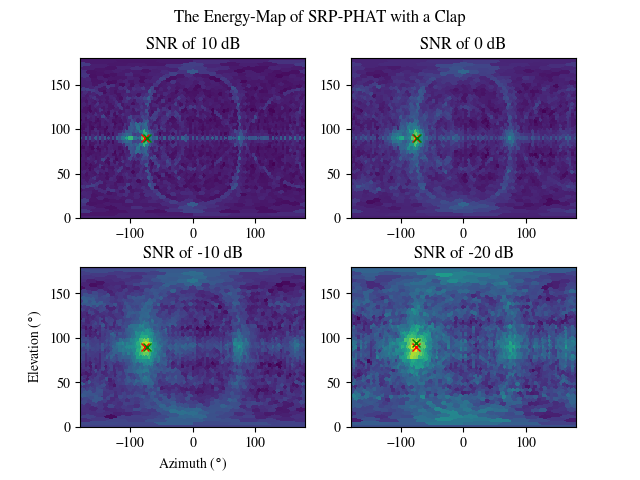
\includegraphics[width=1\textwidth]{../Python/srp_phat/noise/clap/map.png}
\centering
\caption{The energy-map of the SRP-PHAT beamformer is drawn with a clap as the source.}
\label{fig:srp_phat_noise_map_clap}
\centering
\end{figure}

\begin{figure}[H]
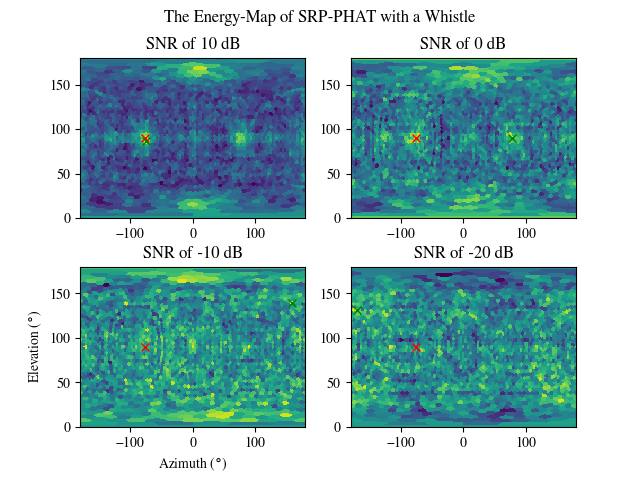
\includegraphics[width=1\textwidth]{../Python/srp_phat/noise/whistle/map.png}
\centering
\caption{The energy-map of the SRP-PHAT beamformer is drawn with a whistle as the source.}
\label{fig:srp_phat_noise_map_whistle}
\centering
\end{figure}

For low noise, there was a very thin and tall peak where the source lied as seen in Figure-\ref{fig:srp_phat_noise_map_clap}. However, as the noise increased, the peak became wider, whilst the rest of the map became more diffused and noisy. This shows how the variance worsened and even how the mean drifted against rising noise since the peak on the energy-map behaves like a probability-distribution. In fact, the whole energy-map is much like a probability-density function.

The effect of noise with a narrowband signal can be seen more easily; the noisy background as much worse in Figure-\ref{fig:srp_phat_noise_map_whistle}.

In some of the maps in Figure-\ref{fig:srp_phat_noise_map_clap}, the side-lobes often associated with beamforming in the literature can be seen; these are seen as subtle curved lines coming from the peak as well as shorter secondary peaks in other directions. Luckily, these do not seem to be too high at least for this geometry.

The energy-map also showed how multiple simultaneous sources could be localised since they would show up as two distinct peaks.

\subsubsection{Discussion}

Indeed, the SRP-PHAT seemed more robust to noise than the other TDOA-based method for the rectangular pyramid array by \cite{chen_sound_2019} although it could not estimate the distance. It did however seem to take twice as long to estimate one direction in the Python simulations; this may be because the method needs to compute for many discrete directions on a search-grid. This apparent slowness can be lessen by pruning obselete directions in the grid, e.g. directly below the array.

The SRP-PHAT was very poor for a narrowband signal such as a whistle. However, this was somewhat expected since it was known that the PHAT worked worse with narrowband signals \cite{valin_localization_2004} \cite{valin_robust_2007}. This may be considered the worst kind of sound and thus set a lower bound of performance; other kinds of sound should fare better. Even still, this can be fine-tuned with some parameters like the sampling rate, the frame-length, the modified spectral weighting. 

\section{Proposed Method}

\subsection{A Further Study into SRP-PHAT}

Given the method used in by some papers \cite{valin_localization_2004}, \cite{valin_robust_2007}, a further study in its parameters such as sampling frequency and how well it works more broadly.

\subsubsection{Experimental Method}

For this set of simulations, the same room was tested as before, but the array is 

\subs

\chapter{Electronics Design}

\section{Overall Design}

Since this system was to be used on a humanoid robot, an embedded solution is needed given that it would draw less power and be smaller and lighter. This makes an added challenge given that most examples in the literature are implemented on either a SOC, a laptop, or even a desktop. Such an embedded solution would behave as a separate process that could handle the high throughput of the microphones and the high computation but then send simple results through USB which would need relatively little throughput.

The biggest factor was the interface between the microphones and the main processor. There were a few potential kinds, namely:
\begin{itemize}
	\item analogue microphones through one or more ADCs,
	\item digital microphones through SPI, I\textsuperscript{2}S, etc.,
	\item and digital microphones through USB.
\end{itemize}
The last was deemed not appropiate since it was not scalable to an embedded processor and might have needed more overhead in the firmware.

\section{Microphones}

The microphones and their respective interface needed:
\begin{itemize}
	\item to be sampled at 48 \si{kHz} at least,
	\item to be omnidirectional,
	\item to be sampled simultaneously exactly at the same time,
	\item to be reasonably robust to electrical interference,
	\item to not take up to much pre-processing to burden the processor's computation,
	\item to be able to handle at least eight microphones on one processor,
	\item to have a good SNR,
	\item to have a good sensitivity,
\end{itemize}
The last two needed not to be too demanding but simply enough so that a wide range of sounds could be heard with enough clarity not to affect the phase.

\subsection{Sensitivity and Dynamic Range}

It is widely known that quiet rooms have a sound-pressure-level of 30 to 40 \si{dB_{SPL}}, and converstions one metre away have that of 60 \si{dB_{SPL}}. Louder environments tend to have level of round 90 \si{dB_{SPL}}. Very loud sounds like a chainsaw about one metre away, aeroplanes, etc. have a level of 120 \si{dB_{SPL}}. 

% http://www.sengpielaudio.com/TableOfSoundPressureLevels.htm

Anything above that is passed the threshold of pain. Although it is not expected that the system must localise sounds of every possible level, it would be best if the system could localise within a range as deep as possible.

However, most microphones would have a noise-floor which is often somewhere between 20 and 40 \si{dB_{SPL}} and is often written as a SNR relative to a single tone of 94 \si{dB_{SPL}} at 1 \si{kHz}. This floor bounds how quiet the sounds can be heard.

% https://www.st.com/resource/en/application_note/an4598-preamplifying-the-analog-output-of-a-mems-microphone-stmicroelectronics.pdf

Furthermore, the sensitivity affects the dynamic range of levels. This is given as the ratio between the output often in volts and the pressure in Pascals, but it is most often written in decibels and for a single tone of 94 \si{dB_{SPL}} at 1 \si{kHz}. The higher the sensitivitiy is, the higher the voltage is. Most electret and MEMS microphones have a sensitivity between -46 and -35 \si{dBV}.

% https://www.analog.com/en/analog-dialogue/articles/understanding-microphone-sensitivity.html#:~:text=Microphone%20sensitivity%20is%20typically%20measured,a%20measure%20of%20its%20sensitivity.

Other specifications of microphones are the total harminic distortion (THD), and the maximum acoustic input. Most common electret and MEMS microphones have a THD  less than 1 \% and a maximum acoustic input of about 120 \si{dB_{SPL}}. However, harmonic distortion might not be a big problem since it does not affect the spectral phase, only the spectral magnitude.

\subsection{Interface}

Small microphones in electronics use many different kinds of communication. The main kinds are:
\begin{itemize}
	\item analogue through an ADC,
	\item pulse-density-modultion (PDM),
	\item I\textsuperscript{2}S, 
	\item SPI,
	\item I\textsuperscript{2}C
\end{itemize}

The first three are the most common, and the last two share similarities with I\textsuperscript{2}S.

\subsubsection{Analogue through an ADC}

The most basic MEMS microphone is one that has its own pre-amplifier and outputs a small yet measurable voltage. This output is often weak and has a higher impedance. So, another amplifier circuit may be needed before an ADC. Indeed, an analogue anti-aliasing filter is also needed which may add complexity to the electronic design.
% https://www.analog.com/media/en/technical-documentation/technical-articles/analog-and-digital-mems-microphone-design-considerations-ms-2472.pdf

Most processors on the market, i.e. microcontrollers, DSPs, etc., have two or three ADCs but with multiplexed channels. However, for each ADC, the channels are sampled sequentially by a single sample-and-hold after the multiplexer. Thus, this means that the channels can never be sampled simultaneously. Therefore, an external ADC chip that can sample simultaneously must be chosen. Such chips can often communicate through either a serial or a parallel interface, e.g. SPI. Given that enough samples from each microphone can be outputed on the interface within a sample-period, then a serial interface should not affect the timing.

For example, eight microphones are sampled at 48 \si{kHz} and at 16 bits by an external ADC chip which communicates through SPI with a clock-frequency of 20 \si{MHz}. The number of needed clock-cycles to output all eight samples is $8\cdot 16 = 128$, and the time to output all is thus:
\begin{equation}
\frac{128}{20 \si{MHz}} = 6.4 \si{\micro s}
\end{equation}
which is less than the sample-period of $1/48 \si{kHz} = 20.8\si{micro s}$ and thus gives enough time to add it to a buffer for example in the processor. Indeed, some external ADC chips such as the one cited allow for multiple serial outputs so that the throughput can be higher.
% AD7606

Otherwise, the simultaneous sampling can be forsaken so that system samples sequentially instead, and the design is simpler, but it is unpredictable how this imprecise sampling will affect the algorithm. It is therefore safer to assume the worst and design the system to sample simultaneously.

\subsubsection{PDM}

PDM microphones have additional circuitry made up of an ADC and modulator. Pulse-density-modulation (PDM) is where the sound-signal is encoded as bits whose density correlates to the sound's amplitude. These bits are output by a given clock-signal. Thus, PDM microphones can be connected to SPI, I\textsuperscript{2}S, and other interfaces on a microcontroller. For example, some STM32s have modules specifically for communicating with PDM microphones that can allow up to eight microphones. At worst, the delay between two channels can be half the clock-cycle which is often in the range of \si{MHz} and thus not too long.

This stream of bits is then filtered, decimated, and converted to a PCM signal of integer values. However, because of this, there may be more computational burden since it has to be done by the processor.

\subsubsection{I\textsuperscript{2}S and Other Serial Interfaces}

Like SPI and I\superscript{2}C, I\textsuperscript{2}S allows a microphone to output a word representing a value on a serial data-line along with a clock-signal. Thus, the data can be output at a much lower rate. Some microcontrollers allow three or four I\textsuperscript{2}S interface, each can allow two microphones. Therefore, some microcontrollers can allow eight microphones in theory. However, there seems to be no guarantee that the samples of each microphone are simultaneous or even near such.

\section{Anti-aliasing Filter}

If an analogue output is to be read by an ADC from the microphone, then an analgoue anti-aliasing filter must be used lest noise and other components of higher frequency in the stop-band are folded back into the pass-band. 

The phase-response should be carefully taken into mind. Although a perfect lienar phase-response is not needed, the phase-response must be consistent between channels, i.e. microphoens, since the GCC-PHAT only takes the relative difference in phase between two such channels. Therefore, components like capacitors must be precise enough to not propogate any variance in the phase-response. On the other hand, the magnitude-response is not too important since GCC-PHAT will whiten the spectrum anyway.

Furthermore, most analogue filters cannot have both a steep roll-off and a good phase-response. Even then, filters of higher order have more components and complexity and can thus lead to inconsistencies between the channels.

Therefore, one solution for example is to have the cut-off of -3 \si{dB} at 10 \si{kHz}\footnote{This is a good compromise in bandwidth since most common sounds lie therewithin, and although humans can theoretically hear sounds above this, most can practically not.}. A second-order filter will then have a cut-off of -40 \si{dB} at 100 \si{kHz} which will give a sampling rate of 200 \si{kSs^{-1}}. However, this will have to be downsampled to 48 \si{kHz} since the simulations have been done with this sampling frequency in mind, and faster sampling tends to worsen the GCC-PHAT.

\section{External ADC Chip}

An external ADC chip is needed that:
\begin{itemize}
	\item can sample at 100 \si{kHz},
	\item can communicate eight samples within one sample-period,
	\item can sample eight channels simultaneously,
	\item and has a reasonably compatible digital interface whether it is serial or parallel.
\end{itemize}

\section{Processor}

The processor can be either a simple micrcontroller or a digital signal processor (DSP); the latter may be more suited to this application. A processor is needed that:
\begin{itemize}
	\item can communicate with an external ADC, or communicate with digital microphones,
	\item has a reasonably high clock-speed,
	\item has hardware-accelerated FFT among other mathematical optimisations,
	\item and can communicate through USB or any other simple interface e.g. UART to send results.
\end{itemize}

\chapter{Conclusion}

After this first semester, the literature-review has mostly been completed and has given a deep insight into existing methods and examples that most relevant to this project and robotics in general. Mostly, signal-processing techniques related to either TDOA, beamforming, and MUSIC have been explored.

Furthermore, simulations have been done to further study the methods and the algorithms. At least two examples have been evaluated in terms of accuracy and precision against noise. Although the TDOA-based method using a rectangular pyramid as described in \cite{chen_sound_2019} is one of the few that estimates distance, it is less robust to noise and thus may likely need improvement. Otherwise, the method of SRP-PHAT mainly inspired by \cite{valin_localization_2004} and \cite{valin_robust_2007} seems to be fairly robust and precise. These simulations will likely help lead to a chosen method for the physical testing and design.

Future work after this semester will be to continue evaluating existing methods and develop a method specific for this project which may be take inspiration from studied methods and even a combination of which. This chosen method will then need to be tested again in simulation. In the next semester of this project, the most important work to be done is to design and implement the physical prototype which will involve a fair deal of consideration. In particular, the embedded programming will need to take into account the computing-time and thus the real-time processing. After a physical prototype has been made, then it must be tested in physical experiments to confirm the performance.

%\chapter{Appendix}
%
%\begin{table}[H]
%\begin{tabular}{c | c c c c}
%\hline
%Paper
%& Type	
%& Method		
%& Result		
%& Sources \\
%\hline
%Valin et al., 2003 \cite{valin_robust_2003}
%& TDOA	
%& GCC-PHAT	
%& 3D angle	
%& single \\
%Hu et al., 2009 \cite{hu_estimation_2009}
%& TDOA
%& ES-GCC	
%& 3D angle	
%& multiple \\
%Chen \& Xu, 2019 \cite{chen_sound_2019}	
%& TDOA
%& GCC-PHAT	
%& full 3D coordinates
%& single \\
%Bechler et al., 2004 \cite{bechler_system_2004}	
%& TDOA
%& GCC-PHAT	
%& full 3D coordinates
%& single \\
%Manamperi et al., 2022 \cite{manamperi_drone_2022}
%& Beamforming
%& SRP-PHAT
%& 3D angle
%& multiple \\
%Valin et al., 2004 \cite{valin_localization_2004}	
%& Beamforming
%& SRP-PHAT
%& 3D angle
%& multiple \\
%Valin et al., 2007 \cite{valin_robust_2007}
%& Beamforming
%& SRP-PHAT	
%& 3D angle
%& multiple \\
%Salvati et al., 2019 \cite{salvati_power_2019}
%& Beamforming
%& DU	
%& 3D angle
%& multiple \\
%Zhang et al., 2021 \cite{zhang_improved_2021}	
%& Beamforming
%& DSB
%& 3D angle
%& multiple \\
%Basiri et al., 2016 \cite{basiri_-board_2016}	
%& Beamforming
%& SRP-PHAT
%& 3D angle	
%& multiple \\
%Ishi et al., 2009 \cite{ishi_evaluation_2009}	
%& MUSIC
%& SEVD
%& 3D angle
%& multiple \\
%Nakamura et al., 2012 \cite{nakamura_real-time_2012}
%& MUSIC
%& GSVD
%& 3D angle
%& multiple \\
%\hline
%\end{tabular}
%\centering
%\caption{The first table of the literature-review.}
%\label{tab:lit_rev_1}
%\centering
%\end{table}
%
%\begin{table}[H]
%\begin{tabular}{c c c c}
%\hline
%Accuracy	
%& Resolution	
%& Microphones
%& Dimensions \\
%\hline
%0.6 - 4.9 \si{\deg} (MSE)
%& ?
%& 8	
%& $0.5\times 0.4\times 0.36$ \si{m} \\
%< 3 \si{\deg} (average error)
%& ?	
%& 8	
%& 0.24 \si{m} overall \\
%0.4 \si{m}, 1.9 \si{\deg} \footnote{distance and azimuth respectively at worst at 6 \si{m} and 10 \si{dB}}
%& ?	
%& 5	
%& 0.35 \si{m} overall \\
%4.957 - 27.21 \si{\e{-3}}{$m^2$} (MSE)
%& ?	
%& 5	
%& 0.48 \si{m} overall \\
%0.05 - 9.43 \si{\deg}	
%& ?	
%& 30
%& ? \\
%100 - 42 \% (success-rate) \footnote{The latter is at worst for speech at 7 \si{m}.}	
%& 2.5 \si{\deg}	
%& 8	
%& $0.5\times 0.4\times 0.36$ \si{m} \\
%1.10 \si{\deg}, 0.89 \si{\deg} (RMSE) \footnote{azimuth and elevation respectively}	
%& 2.5 \si{\deg}	
%& 8	
%& cube 15.5 \si{cm} wide \\
%2.5 \si{\deg} (RMSE) \footnote{at worst for a single source at -10 \si{dB}}	
%& 5 \si{\deg}	
%& 8	
%& circle 40 \si{cm} wide \\
%2 \si{\deg} at worst
%& ?	
%& 16
%& two concentric circles, 20 and 40 \si{cm} wide \\
%1.39 \si{\deg} (RMSE) \footnote{for a single source}	
%& ?	
%& 4	
%& T-shape \\
%~80 \% (success-rate)
%& 5 \si{\deg}
%& 14
%& 40 \si{cm} overall \\
%1 - 10 \si{\deg} \footnote{at worst for an azimuth of 120 \si{\deg}}	
%& 1 \si{\deg}	
%& 8	
%& circle \\
%\hline
%\end{tabular}
%\centering
%\caption{The first table of the literature-review.}
%\label{tab:lit_rev_1}
%\centering
%\end{table}

%\nocite{*}

\bibliographystyle{plain}
\bibliography{./zotero}

%\begin{figure}[!h]
%\includegraphics[width=1\textwidth]{image.png}
%\centering
%\caption{Caption,}
%\label{fig:image}
%\centering
%\end{figure}

%\includepdf[pages=-,pagecommand={},angle=90,width=\textwidth]{controller_1.pdf}
%\includepdf[pages=-,pagecommand={},angle=90,width=\textwidth]{regulator_1.pdf}
%\includepdf[pages=-,pagecommand={},angle=90,width=\textwidth]{timer_1.pdf}


\end{document}
